\documentclass[12 pt]{article}
\usepackage[utf8]{inputenc}
\usepackage[english]{babel}
\title{A New Approach to Artificial Neural Networks}
\author{Azmi C. Özgen}
\usepackage{setspace}
% \usepackage[top=2.5cm, bottom=2.5cm, left=4cm, right=2.5cm]{geometry}
\usepackage{geometry}
 \geometry{
 a4paper,
 % total={210mm,297mm},
 left=40mm,
 right=25mm,
 top=25mm,
 bottom=25mm,
 }
\usepackage{titlesec}
\usepackage{times} %Times New Roman
\usepackage{amssymb,amsmath}
\usepackage{ifxetex,ifluatex}
\usepackage{multicol}
\usepackage{fixltx2e} % provides \textsubscript
\ifnum 0\ifxetex 1\fi\ifluatex 1\fi=0 % if pdftex
  \usepackage[T1]{fontenc}
  \usepackage[utf8]{inputenc}
\else % if luatex or xelatex
  \ifxetex
    \usepackage{mathspec}
    \usepackage{xltxtra,xunicode}
  \else
    \usepackage{fontspec}
  \fi
  \defaultfontfeatures{Mapping=tex-text,Scale=MatchLowercase}
  \newcommand{\euro}{€}
\fi
% use upquote if available, for straight quotes in verbatim environments
\IfFileExists{upquote.sty}{\usepackage{upquote}}{}
% use microtype if available
\IfFileExists{microtype.sty}{\usepackage{microtype}}{}
\usepackage{graphicx}
\makeatletter
\def\maxwidth{\ifdim\Gin@nat@width>\linewidth\linewidth\else\Gin@nat@width\fi}
\def\maxheight{\ifdim\Gin@nat@height>\textheight\textheight\else\Gin@nat@height\fi}
\makeatother
% Scale images if necessary, so that they will not overflow the page
% margins by default, and it is still possible to overwrite the defaults
% using explicit options in \includegraphics[width, height, ...]{}
\setkeys{Gin}{width=\maxwidth,height=\maxheight,keepaspectratio}
\ifxetex
  \usepackage[setpagesize=false, % page size defined by xetex
              unicode=false, % unicode breaks when used with xetex
              xetex]{hyperref}
\else
  \usepackage[unicode=true]{hyperref}
\fi
\hypersetup{breaklinks=true,
            bookmarks=true,
            pdfauthor={Azmi C. Özgen},
            pdftitle={A New Approach to Artificial Neural Networks},
            colorlinks=true,
            citecolor=blue,
            urlcolor=blue,
            linkcolor=black,
            pdfborder={0 0 0}}
\urlstyle{same}  % don't use monospace font for urls
\setlength{\parindent}{0pt}
\setlength{\parskip}{6pt plus 2pt minus 1pt}
\setlength{\emergencystretch}{3em}  % prevent overfull lines
\setcounter{secnumdepth}{0}

\begin{document}
\onehalfspacing
\pagestyle{plain}
\pagenumbering{roman}
\setcounter{page}{1}
\tableofcontents
\newpage
\begin{abstract}
    \thispagestyle{plain}
    \setcounter{page}{3}
    Machine learning is a growing area in computer science. Neural networks
    is very popular subdomain of it. This project generally covers the work
    of M. Nielsen and his book Neural Networks and Deep Learning. We
    will first introduce neual networks and then apply it to a generic
    problem which is called classifying handwritten digits.
\end{abstract}
\newpage

\section{Acknowledgements}
I would like to thank first my advisor A. Levent Subaşı for his insightful
comments. And I am grateful Berkin Malkoç, Melih Taşdizen and Kürşat Aker
for their precious support. Also, I thank my fellow mates Mustafa Can Uslu,
Onur Kaplan and Ceren Güzelgün for their fabulous friendships. Last but
not the least, I thank to my family for their endless support.
\newpage

\section{Abbreviations}
    MLP   &  Multilayer Perceptron \\
    MNIST &  Mixed National Institute of Standards and Technology database \\
    MSE   &  Mean Squared Error \\
\newpage

\section{1. Introduction}\label{introduction}
\pagenumbering{arabic}
\setcounter{page}{1}

The idea of neural networks is to take a large number of dataset known
as training examples, and then develop a system which can learn from
those training examples. In other words, the neural network uses the
examples to automatically infer rules for recognizing other unknown
examples. Furthermore, by increasing the number of training examples,
the network can learn more about handwriting, and so improve its
accuracy.

There are just 100 training digits below, perhaps we could build a
better handwriting recognizer by using thousands or even millions or
billions of training examples.

\begin{figure}[htp]
\centering
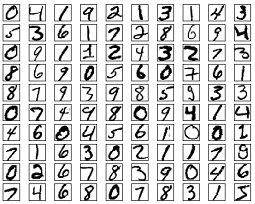
\includegraphics{./figs/mnist_100_digits.png}
\caption{100 Handwritten Digits}
\end{figure}

This project is concerned with write a computer program implementing a
neural network that learns to recognize handwritten digits and generally
covers the work of M. Nielsen and his book Neural Networks and Deep Learning.\cite{ref1}

Along the way there are many key ideas about neural networks, including
two important types of artificial neuron (the perceptron and the sigmoid
neuron), and the standard learning algorithm for neural networks, known
as stochastic gradient descent.

\subsection{1.1. Perceptrons}\label{perceptrons}

Perceptron is a type of artificial neuron. Perceptrons were developed in
the 1950s and 1960s by the scientist Frank Rosenblatt, inspired by
earlier work by Warren McCulloch and Walter Pitts. Today, it's more
common to use other models of artificial neurons - in this book, and in
much modern work on neural networks, the main neuron model used is one
called the sigmoid neuron.

A perceptron takes several binary inputs, $ x_1, x_2, \ldots{}, $
and produces a single binary output:

\begin{figure}[htp]
\centering
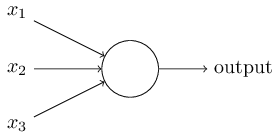
\includegraphics[width=0.5\textwidth]{./figs/tikz0.png}
\caption{Perceptron}
\end{figure}

In general it could have more or fewer inputs. Rosenblatt proposed a
simple rule to compute the output. He introduced weights,
$ w_1,w_2,\ldots{}, $ real numbers expressing the importance of the respective
inputs to the output. The neuron's output, 0 or 1, is determined by
whether the weighted sum $ \sum_j w_j x_j $ is less than or
greater than some threshold value. Just like the weights, the threshold
is a real number which is a parameter of the neuron. To put it in more
precise algebraic terms:

\begin{equation}
    output =
    \begin{cases}
        0,& if \hspace{0.5 cm} \sum_j\ w_jx_j \leqslant threshold \\
        1,& if \hspace{0.5 cm} \sum_j\ w_jx_j > threshold
    \end{cases}
\end{equation}

That's all there is to how a perceptron works!

That's the basic mathematical model. A way you can think about the
perceptron is that it's a device that makes decisions by weighing up
evidence.

Obviously, the perceptron isn't a complete model of human
decision-making! But what the example illustrates is how a perceptron
can weigh up different kinds of evidence in order to make decisions. And
it should seem plausible that a complex network of perceptrons could
make quite subtle decisions:

\begin{figure}[htp]
\centering
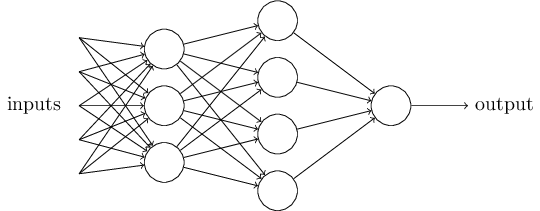
\includegraphics[width=0.5\textwidth]{./figs/tikz1.png}
\caption{Multilayer Perceptron (MLP)}
\end{figure}

In this network, the first column of perceptrons - the first layer of
perceptrons - is making three very simple decisions, by weighing the
input evidence. What about the perceptrons in the second layer? Each of
those perceptrons is making a decision by weighing up the results from
the first layer of decision-making. In this way a perceptron in the
second layer can make a decision at a more complex and more abstract
level than perceptrons in the first layer. And even more complex
decisions can be made by the perceptron in the third layer. In this way,
a many-layer network of perceptrons can engage in sophisticated decision
making.

In the first example, it is defined perceptrons has just a single
output. In the network above the perceptrons look like they have
multiple outputs. In fact, they're still single output. The multiple
output arrows are merely a useful way of indicating that the output from
a perceptron is being used as the input to several other perceptrons.
It's less unwieldy than drawing a single output line which then splits.

Let's simplify the way we describe perceptrons. The first change is to
write $ \sum_j w_j x_j $ as a dot product, $ w \cdot x
\equiv \sum_j w_j x_j $, where $ w $ and $ x $ are vectors whose components are
the weights and inputs, respectively.
The second change is to move the threshold to the other side of the inequality,
and to replace it by what's known as the perceptron's bias,
$ b \equiv -threshold. $ Using the bias instead of the threshold, the
perceptron rule can be rewritten:

\begin{equation}
    output =
    \begin{cases}
        0,& if \hspace{0.5 cm} w \cdot x + b \leq 0 \\
        1,& if \hspace{0.5 cm} w \cdot x + b > 0
    \end{cases}
\end{equation}

You can think of the bias as a measure of how easy it is to get the
perceptron to output a 1. Or to put it in more biological terms, the
bias is a measure of how easy it is to get the perceptron to fire. For a
perceptron with a really big bias, it's extremely easy for the
perceptron to output a 1. But if the bias is very negative, then it's
difficult for the perceptron to output a 1.

\subsection{1.2. Sigmoid neurons}
\label{sigmoid-neurons}

Suppose we have a network of perceptrons that we'd like to use to learn
to solve some problem. For example, the inputs to the network might be
the raw pixel data from a scanned, handwritten image of a digit. And
we'd like the network to learn weights and biases so that the output
from the network correctly classifies the digit. To see how learning
might work, suppose we make a small change in some weight (or bias) in
the network. What we'd like is for this small change in weight to cause
only a small corresponding change in the output from the network. As
we'll see in a moment, this property will make learning possible.
Schematically, here's what we want (obviously this network is too simple
to do handwriting recognition!):

\begin{figure}[htp]
\centering
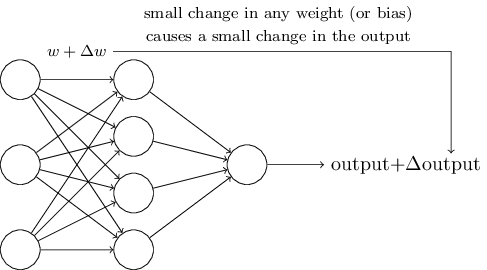
\includegraphics[width=0.5\textwidth]{./figs/tikz8.png}
\caption{Effects of changing weights to the output}
\end{figure}

If it were true that a small change in a weight (or bias) causes only a
small change in output, then we could use this fact to modify the
weights and biases to get our network to behave more in the manner we
want.

The problem is that this isn't what happens when our network contains
perceptrons. In fact, a small change in the weights or bias of any
single perceptron in the network can sometimes cause the output of that
perceptron to completely flip, say from 0 to 1. That flip may then cause
the behaviour of the rest of the network to completely change in some
very complicated way.

We can overcome this problem by introducing a new type of artificial
neuron called a sigmoid neuron. Sigmoid neurons are similar to
perceptrons, but modified so that small changes in their weights and
bias cause only a small change in their output. That's the crucial fact
which will allow a network of sigmoid neurons to learn.

Okay, let me describe the sigmoid neuron. We'll depict sigmoid neurons
in the same way we depicted perceptrons. Just like a perceptron, the
sigmoid neuron has inputs, $ x_1, x_2, \ldots{} $ But instead of
being just 0 or 1, these inputs can also take on any values between 0
and 1. So, for instance, $ 0.638 $ is a valid input for a sigmoid
neuron. Also just like a perceptron, the sigmoid neuron has weights for
each input, $ w_1, w_2, \ldots{} $ and an overall bias, $ b
$. But the output is not 0 or 1. Instead, it's $ \sigma (w \cdot x + b)
$, where $ \sigma $ is called the sigmoid function - sometimes called
logistic function - and this new class of neurons called sigmoid neurons
or logistic neurons. and is defined by:

\begin{equation}
    \sigma(z) \equiv \frac{1}{1 + e^{-z}}
\end{equation}

The output of a sigmoid neuron with inputs $ x_1, x_2, \ldots{} $
weights $ w_1, w_2, \ldots{} $ and bias $ b $ is

\begin{equation}
    \frac {1}{1 + exp(−\sum_j w_j x_j − b)}
\end{equation}

To understand the similarity to the perceptron model, suppose $ z
\equiv w \cdot x + b $ is a large positive number. Then $ e ^ {−z}
\approx 0 $ and so $ \sigma(z) \approx 1 $ just as it would
have been for a perceptron. Suppose on the other hand that $ z = w
\cdot x + b $ is very negative. Then $ e ^{−z} \to \infty $,
and $ \sigma(z) \approx 0 $ like a perceptron.

\begin{figure}[htp]
\centering
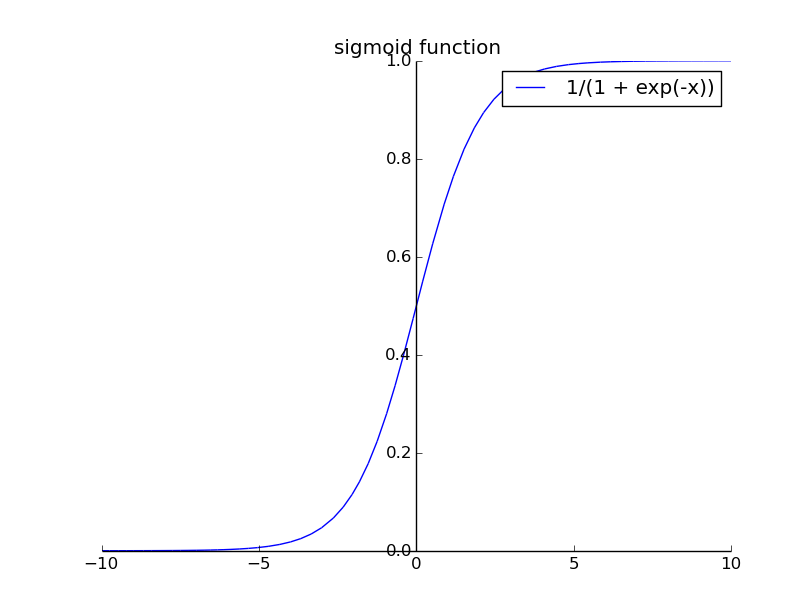
\includegraphics[width=0.7\textwidth]{./figs/sigmoid_function.png}
\caption{Sigmoid function}
\end{figure}

This shape is a smoothed out version of a step function or Heaviside
step function:

\begin{figure}[htp]
\centering
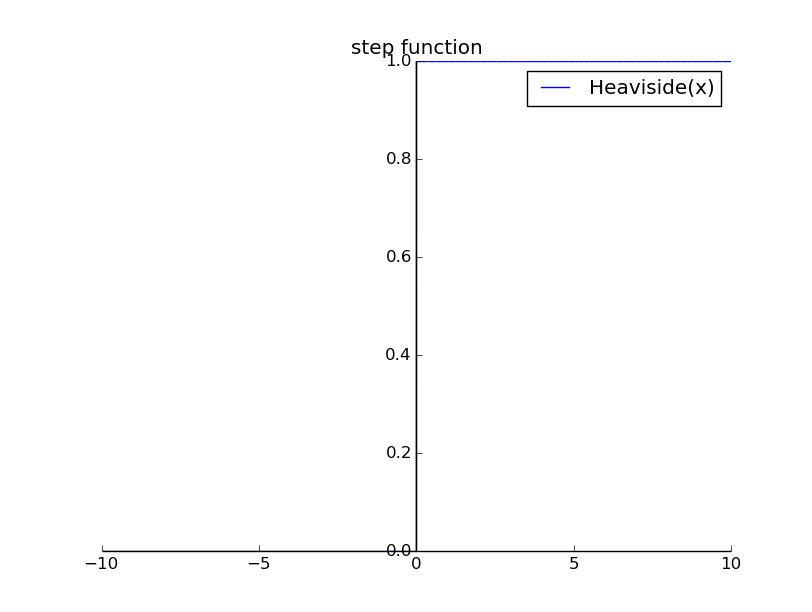
\includegraphics[width=0.7\textwidth]{./figs/step_function.png}
\caption{Step function}
\end{figure}

If $ \sigma $ had in fact been a step function, then the sigmoid
neuron would be a perceptron, since the output would be 1 or 0 depending
on whether $ w \cdot x + b $ was positive or negative. Actually, when
$ w \cdot x + b = 0 $ the perceptron outputs 0, while the step
function outputs 1. So, strictly speaking, we would need to modify the
step function at that one point.

By using the actual $ \sigma $ function we get, a smoothed out
perceptron. The smoothness of $ \sigma $ means that small changes
$ \Delta w_j $ in the weights and $ \Delta b $ in the bias will
produce a small change $ \Delta output $ in the output from the
neuron. In fact, calculus tells us that $ \Delta output $ is well
approximated by

\begin{equation}
    \Delta output \approx \sum_j
    \frac {\partial \ output}{\partial w_j} \Delta w_j +
    \frac {\partial \ output}{\partial b} \Delta b
\end{equation}

where the sum is over all the weights, $ w_j $, and $
\frac{\partial \ output}{\partial w_j} $ and $
\frac{\partial \ output}{\partial b} $ denote partial derivatives of
the output with respect to $ w_j $ and $ b $, respectively. So
while sigmoid neurons have much of the same qualitative behaviour as
perceptrons, they make it much easier to figure out how changing the
weights and biases will change the output.

If it's the shape of $ \sigma $ which really matters, and not its
exact form, then why use the particular form used for $ \sigma $ ? In
fact, there are other activation functions as well. The main thing that
changes when we use a different activation function is that the
particular values for the partial derivatives in Equation (5) change. It
turns out that when we compute those partial derivatives, using $
\sigma $ will simplify the algebra.

\begin{equation}
    \begin{split}
        \frac{d\sigma}{dz} & = \left({1 - \frac{1}{1 + e ^ {-z}}}\right)
        \left(\frac{1}{1 + e ^ {-z}}\right)\\
        & = (1 - \sigma)\sigma
    \end{split}
\end{equation}

\subsection{1.3. The architecture of neural networks}
\label{the-architecture-of-neural-networks}

Suppose we have the network:

\newpage
\begin{figure}[htp]
\centering
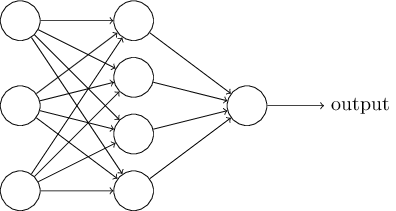
\includegraphics[width=0.5\textwidth]{./figs/tikz10.png}
\caption{Simple architecture}
\end{figure}

As mentioned earlier, the leftmost layer in this network is called the
input layer, and the neurons within the layer are called input neurons.
The rightmost or output layer contains the output neurons, or, as in
this case, a single output neuron. The middle layer is called a hidden
layer, since the neurons in this layer are neither inputs nor outputs.
The network above has just a single hidden layer, but some networks have
multiple hidden layers. For example, the following four-layer network
has two hidden layers:

\begin{figure}[htp]
\centering
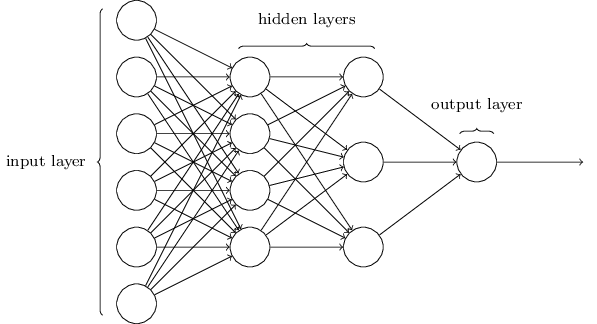
\includegraphics[width=0.5\textwidth]{./figs/tikz11.png}
\caption{Layers}
\end{figure}

Somewhat confusingly, and for historical reasons, such multiple layer
networks are sometimes called multilayer perceptrons or MLPs, despite
being made up of sigmoid neurons, not perceptrons. It is not going to be
used the MLP terminology in this article, since it is confusing.

There can be quite an art to the design of the hidden layers. Neural
networks researchers have developed many design heuristics for the
hidden layers, which help people get the behaviour they want out of
their nets. For example, such heuristics can be used to help determine
how to trade off the number of hidden layers against the time required
to train the network.

Up to now, we've been discussing neural networks where the output from
one layer is used as input to the next layer. Such networks are called
feedforward neural networks. This means there are no loops in the
network - no feedback-. Loops would be problematic in for example
sigmoid neurons because of the inputs would depend on the outputs.
However, there are other models of artificial neural networks in which
feedback loops are possible. These models are called recurrent neural
networks. The idea in these models is to have neurons which fire for
some limited duration of time, before becoming quiescent. That firing
can stimulate other neurons, which may fire a little while later, also
for a limited duration. That causes still more neurons to fire, and so
over time we get a cascade of neurons firing. Loops don't cause problems
in such a model, since a neuron's output only affects its input at some
later time, not instantaneously.

Recurrent neural nets have been less influential than feedforward
networks, in part because the learning algorithms for recurrent nets are
(at least to date) less powerful. But recurrent networks are still
extremely interesting. They're much closer in spirit to how our brains
work than feedforward networks. And it's possible that recurrent
networks can solve important problems which can only be solved with
great difficulty by feedforward networks.

\subsection{1.4. A simple network to classify handwritten digits}
\label{a-simple-network-to-classify-handwritten-digits}

We can split the problem of recognizing handwritten digits into two
sub-problems. First, we'd like a way of breaking an image containing
many digits into a sequence of separate images, each containing a single
digit.

\begin{figure}[htp]
\centering
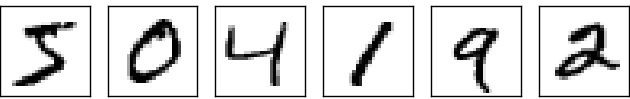
\includegraphics[width=0.5\textwidth]{./figs/digits_separate.png}
\caption{Seperate digits}
\end{figure}

Once the image has been segmented, the program then needs to classify
each individual digit. We will focus on writing a program to classify
individual digits..

To recognize individual digits we will use a three-layer neural network:

\begin{figure}[htp]
\centering
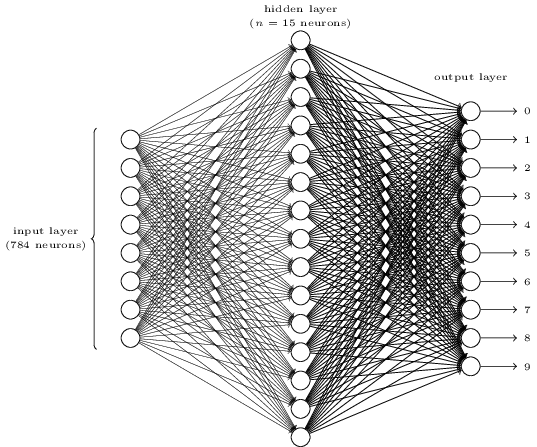
\includegraphics[width=0.5\textwidth]{./figs/tikz12.png}
\caption{Three layered feedforward network}
\end{figure}

As discussed in the next section, our training data for the network will
consist of many 28 by 28 pixel images of scanned handwritten digts, and
so the input layer contains $ 784 = 28 \times 28 $ neurons. The input
pixels are grayscale, with a value of 0.0 representing white, a value of
$ 1.0 $ representing black, and in between values representing gradually
darkening shades of grey.

The second layer of the network is a hidden layer. We denote the number
of neurons in this hidden layer by n, and we'll experiment with
different values for n.

Why we use 10 output neurons. After all, the goal of the network is to
tell us which digit $ (0, 1, 2, \ldots{}, 9) $ corresponds to the
input image. A seemingly natural way of doing that is to use just 4
output neurons, treating each neuron as taking on a binary value,
depending on whether the neuron's output is closer to 0 or to 1. Four
neurons are enough to encode the answer, since $ 2 ^ 4 = 16 $ is
more than 10 possible values for the input digit. Why should our network
use 10 neurons instead? The ultimate justification is empirical. We can
try out both network designs, and it turns out that, for this particular
problem, the network with 10 output neurons learns to recognize digits
better than the network with 4 output neurons. But that leaves us
wondering why using 10 output neurons works better?

\begin{figure}[htp]
\centering
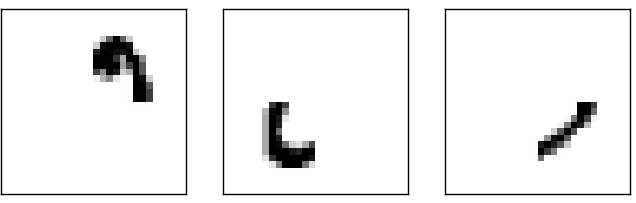
\includegraphics[width=0.5\textwidth]{./figs/mnist_other_features.png}
\caption{Some parts of number 0}
\end{figure}

First neuron in the hidden layer may detect just whether or not an image
like the above is present. If we had 4 outputs, then the first output
neuron would be trying to decide what the most significant bit of the
digit was. And there's no easy way to relate that most significant bit
to simple shapes like those shown above. However there could be always
such structures with 4 neurons at the output so that net were more
efficient. Now, with all that said, this is all just a heuristic.

\subsection{1.5. Learning with gradient descent}
\label{learning-with-gradient-descent}

Now the first thing we'll need is a data set to learn from so-called
training data set. We'll use the MNIST data set which contains
tens of thousands of scanned images of handwritten digits, together with
their correct classifications. Images are the same as used before.

\begin{figure}[htp]
\centering
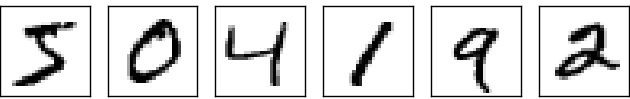
\includegraphics[width=0.5\textwidth]{./figs/digits_separate.png}
\caption{MNIST data set samples}
\end{figure}

The MNIST data comes in two parts. The first part contains 60,000 images
to be used as training data. These images are scanned handwriting
samples from 250 people, half of whom were US Census Bureau employees,
and half of whom were high school students. The images are grayscale and
28 by 28 pixels in size. The second part of the MNIST data set is 10,000
images to be used as test data. Again, these are 28 by 28 grayscale
images. We'll use the test data to evaluate how well our neural network
has learned to recognize digits. To make this a good test of
performance, the test data was taken from a different set of 250 people
than the original training data (albeit still a group split between
Census Bureau employees and high school students). This helps give us
confidence that our system can recognize digits from people whose
writing it didn't see during training.

We'll use the notation $ x $ to denote a training input. It'll be
convenient to regard each training input $ x $ as a $ 28 \times 28 =
784 $ dimensional vector. Each entry in the vector represents the gray
value for a single pixel in the image. We'll denote the corresponding
desired output by $ y = y(x) $, where $ y $ is a 10-dimensional
vector. For example, if a particular training image, $ x $,
depicts a 6, then $ y(x)=(0,0,0,0,0,0,1,0,0,0) ^ T $ is the
desired output from the network. Note that $ T $ here is the transpose
operation, turning a row vector into an ordinary (column) vector.

What we'd like is an algorithm which lets us find weights and biases so
that the output from the network approximates $ y(x) $ for all
training inputs $ x $. To quantify how well we're achieving this goal
we define a cost function. Sometimes referred to as a loss or objective
function.

\begin{equation}
    C(w, \ b)\equiv\frac{1}{2n}\sum_x ||y(x) - a||^2
\end{equation}

Here, $ w $ denotes the collection of all weights in the network, $ b $
all the biases, $ n $ is the total number of training inputs, $ a $
is the vector of outputs from the network when $ x $ is input, and
the sum is over all training inputs, x. Of course, the output $ a $
depends on $ x, w $ and $ b $. The notation
$ ||v|| $ just denotes the usual length function for a vector $ v $.
We'll call $ C $ the quadratic cost function; it's also sometimes
known as the mean squared error or just MSE.
$ C(w, \ b) $ is non-negative, since every term in the sum is
non-negative. Furthermore, the cost $ C(w, \ b) $ precisely when $ y(x) $
is approximately equal to the output, $ a $,
for all training inputs, $ x $.
So our training algorithm has done a good job if it can find weights and biases
so that $ C(w, \ b) \approx 0 $. By contrast, it's not doing so well when $ C(w,\ b) $
is large - that would mean that $ y(x) $ is not close to the
output a for a large number of inputs. So the aim of our training
algorithm will be to minimize the cost $ C(w, \ b) $ as a function of
the weights and biases.

Okay, let's suppose we're trying to minimize some function, $ C(v) $.
This could be any real-valued function of many variables, $ v = v_1, v_2, \ldots{} $

\begin{figure}[htp]
\centering
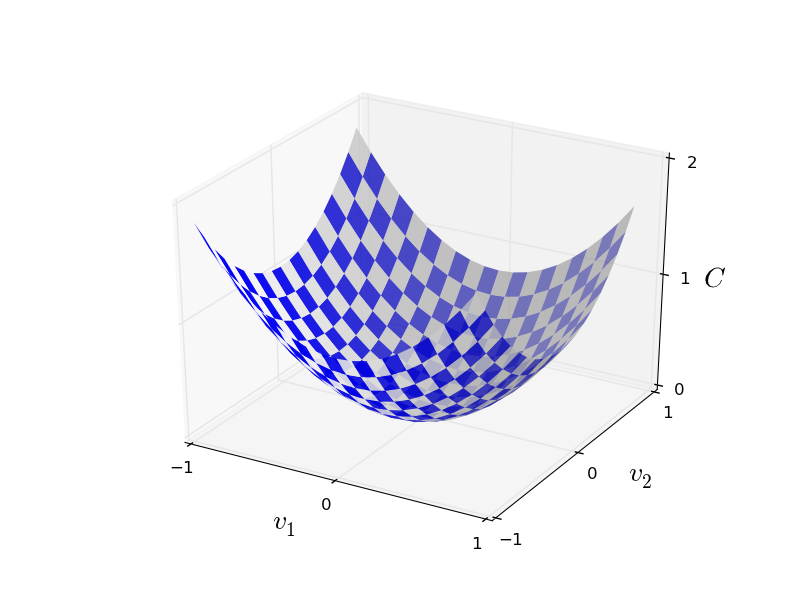
\includegraphics[width=0.7\textwidth]{./figs/valley.png}
\caption{Sample cost function with double variables}
\end{figure}

What we'd like is to find where $ C $ achieves its global minimum. One
way of attacking the problem is to use calculus to try to find the
minimum analytically. With some luck that might work when $ C $ is a
function of just one or a few variables. But it'll turn into a nightmare
when we have many more variables. And for neural networks we'll often
want far more variables - the biggest neural networks have cost
functions which depend on billions of weights and biases in an extremely
complicated way. Using calculus to minimize that just won't work! We
start by thinking of our function as a kind of a valley. And we imagine
a ball rolling down the slope of the valley. Our everyday experience
tells us that the ball will eventually roll to the bottom of the valley.

Let's think about what happens when we move the ball a small amount
$ \Delta v_1 $ in the $ v_1 $ direction, and a small amount
$ \Delta v_2 $ in the $ v_2 $ direction. Calculus tells us that C
changes as follows:

\begin{equation}
    \Delta C \approx \frac {\partial C}{\partial v_1} \Delta v_1 +
    \frac{\partial C}{\partial v_2} \Delta v_2
\end{equation}

We're going to find a way of choosing $ \Delta v_1 $ and $
\Delta v_2 $ so as to make $ \Delta C $ negative; i.e., we'll choose
them so the ball is rolling down into the valley. To figure out how to
make such a choice it helps to define $ \Delta v $ to be the vector of
changes in $ v $, $ \Delta v \equiv (\Delta v_1, \ \Delta v_2)^T $.
We denote the gradient vector by $ \nabla C $, i.e.:

\begin{equation}
    \nabla C \equiv \left( \frac{\partial C}{\partial v_1}, \ \frac{\partial C}
    {\partial v_2} \right)^T
\end{equation}

More generally, if $ C $ is function of $ m $ variables,

\begin{equation}
    \nabla C \equiv \left( \frac{\partial C}{\partial v_1},
    \frac{\partial C}{\partial v_2}, \ ..., \ \frac{\partial C}
    {\partial v_m} \right)^T
\end{equation}

With these definitions, the expression (8) for $ \Delta C $ can be
rewritten as

\begin{equation}
    \Delta C \approx \nabla C ⋅ \Delta v
\end{equation}

In particular, suppose we choose,

\begin{equation}
    \Delta v = −\eta \nabla C
\end{equation}

where $ \eta $ is a small, positive parameter (known as the learning
rate). Then Equation (11) becomes

\begin{equation}
     \Delta C \approx −\eta \nabla C \cdot \nabla C = −\eta || \nabla C|| ^
     2
\end{equation}

This guarantees that $ \Delta C \leq 0 $, i.e., $ C $ will always
decrease. This is exactly the property we wanted! And so we'll take
Equation (12) to define the ``law of motion'' for the ball in our
gradient descent algorithm. That is, we'll use Equation (12) to compute
a value for $ \Delta v $, then move the ball's position v by that
amount:

\begin{equation}
    v \to v' = v − \eta \nabla C
\end{equation}

Then we'll use this update rule again, to make another move. If we keep
doing this, over and over, we'll keep decreasing $ C $ until - we hope
- we reach a global minimum.

Summing up, the way the gradient descent algorithm works is to
repeatedly compute the gradient $ \nabla C $, and then to move in the
opposite direction, ``falling down'' the slope of the valley.

To make gradient descent work correctly, we need to choose the learning
rate $ \eta $ to be small enough that Equation (12) is a good
approximation. If we don't, we might end up with $ \Delta C
\textgreater{} 0 $, which obviously would not be good!
At the same time, we don't want $ \eta $ to be too small,
since that will make the changes $ \Delta v $ tiny,
and thus the gradient descent algorithm will work very slowly.

Unfortunately, this rule does not always work - several things can go
wrong and prevent gradient descent from finding the global minimum of
$ C $, a point we'll return to explore in later chapters. But, in
practice gradient descent often works extremely well, and in neural
networks we'll find that it's a powerful way of minimizing the cost
function, and so helping the net learn.

How can we apply gradient descent to learn in a neural network? The idea
is to use gradient descent to find the weights $ w_k $ and biases
$ b_l $ which minimize the cost in Equation (7). To see how this works,
let's restate the gradient descent update rule, with the weights and
biases replacing the variables $ v_j $.

\begin{equation}
    \begin{split}
        w_k \to w_k' &= w_k − \eta \frac{\partial C}{\partial w_k} \\
        b_l \to b_l' &= b_l − \eta \frac{\partial C}{\partial b_l}
    \end{split}
\end{equation}

By repeatedly applying this update rule we can ``roll down the hill'',
and hopefully find a minimum of the cost function. In other words, this
is a rule which can be used to learn in a neural network.

Notice that this cost function has the form $ C = \frac{1}{n}
\sum_x C_x $, that is, it's an average over costs $ C_x \equiv
\frac{||y(x) - a|| ^ 2}{2} $ for individual training examples. In
practice, to compute the gradient $ \nabla C $ we need to compute the
gradients $ \nabla C_x $ separately for each training input,
$ x $, and then average them, $ \nabla C = \frac{1}{n} \sum_x
\nabla C_x $. Unfortunately, when the number of training inputs is very
large this can take a long time, and learning thus occurs slowly.

An idea called stochastic gradient descent can be used to speed up
learning. The idea is to estimate the gradient $ \nabla C $ by
computing $ \nabla C_x $ for a small sample of randomly chosen
training inputs. By averaging over this small sample it turns out that
we can quickly get a good estimate of the true gradient $ \nabla C $,
and this helps speed up gradient descent, and thus learning.

To make these ideas more precise, stochastic gradient descent works by
randomly picking out a small number $ m $ of randomly chosen training
inputs. We'll label those random training inputs $ X_1, X_2,\ldots{},
X_m $ and refer to them as a mini-batch.

\begin{equation}
    \nabla C \approx \frac{1}{m} \sum_{j = 1} \nabla C_{X_j}
\end{equation}

Equation (16) depicts that overall gradient can be estimated just by
randomly chosen mini-batch. And updating weights and biases is like
below

\begin{equation}
    \begin{split}
        w_k \to w_k' &= w_k − \frac{\eta}{m} \sum_j \frac{\partial C_{X_j}}
        {\partial w_k} \\
        b_l \to b_l' &= b_l − \frac{\eta}{m} \sum_j \frac{\partial C_{X_j}}
        {\partial b_l}
    \end{split}
\end{equation}

where the sums are over all the training examples $ X_j $ in the
current mini-batch. Then we pick out another randomly chosen mini-batch
and train with those. And so on, until we've exhausted the training
inputs, which is said to complete an epoch of training. At that point we
start over with a new training epoch.

It's much easier to sample a small mini-batch than it is to apply
gradient descent to the full batch. For example, if we have a training
set of size $ n = 60,000 $, as in MNIST, and choose a mini-batch size of
(say) $ m = 10 $, this means we'll get a factor of 6,000 speedup in
estimating the gradient! Of course, the estimate won't be perfect -
there will be statistical fluctuations - but it doesn't need to be perfect:
all we really care about is moving in a general direction that will help
decrease C, and that means we don't need an exact computation of the gradient.
In practice, stochastic gradient descent is a commonly used and powerful
technique for learning in neural networks.

\subsection{1.6. Implementing our network to classify digits}
\label{implementing-our-network-to-classify-digits}

Get the codes from
https://github.com/mnielsen/neural-networks-and-deep-learning\cite{ref2}

First MNIST must be loaded.

\begin{verbatim}
>>>import mnist_loader
>>>training_data, validation_data, test_data = \
mnist_loader.load_data_wrapper()
\end{verbatim}

Then,

\begin{verbatim}
>>>import network
>>>net = network.Network([784, 30, 10])
\end{verbatim}

Finally, we'll use stochastic gradient descent to learn from the MNIST
training data over 30 epochs, with a mini-batch size of 10, and a
learning rate of $ \eta $ = 3.0,

\begin{verbatim}
>>>net.SGD(training_data,30,10,3.0,test_data=test_data)
\end{verbatim}

The results are,

\begin{verbatim}
Epoch 0: 9129 / 10000
Epoch 1: 9295 / 10000
Epoch 2: 9348 / 10000
...
Epoch 27: 9528 / 10000
Epoch 28: 9542 / 10000
Epoch 29: 9534 / 10000
\end{verbatim}

That is, the trained network gives us a classification rate of about 95
percent - 95.42 percent at its peak (``Epoch 28'')! That's quite
encouraging as a first attempt. However, that if you run the code then
your results are not necessarily going to be quite the same as mine,
since we'll be initializing our network using (different) random weights
and biases.

Choosing the learning rate $ \eta $ too low i.e. $ \eta = 0.001
$, causes slowly convergence and you may not get good results in reasonable epoch numbers like 100 epochs. On the other hand choosing $
\eta $ too high i.e. $ \eta = 100 $ causes to divergence continuously
and you get very low accurate results.

Learning rate, epoch number, mini batch-size etc. are hyper parameters.
You can adjust these parameters and may get better and faster results.

\section{2. How the backpropagation algorithm works}
\label{how-the-backpropagation-algorithm-works}

The backpropagation algorithm was originally introduced in the 1970s,
but its importance wasn't fully appreciated until a famous 1986 paper by
David Rumelhart, Geoffrey Hinton, and Ronald Williams. That paper
describes several neural networks where backpropagation works far faster
than earlier approaches to learning, making it possible to use neural
nets to solve problems which had previously been insoluble. Today, the
backpropagation algorithm is the workhorse of learning in neural
networks.

\subsection{2.1. A fast matrix-based approach to computing the
output from a neural network}
\label{warm-up-a-fast-matrix-based-approach-to-computing-the-output-from-a-neural-network}

We'll use $ w^l_{jk} $ to denote the weight for the connection
from the $ k^{th} $ neuron in the $ (l − 1)^{th} $ layer
to the $ j^{th} $ neuron in the $ l^{th} $ layer. So, for
example, the diagram below shows the weight on a connection from the
fourth neuron in the second layer to the second neuron in the third
layer of a network:

\begin{figure}[htp]
\centering
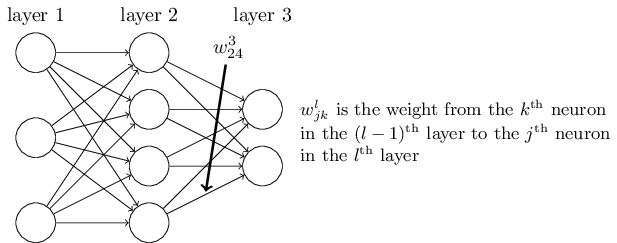
\includegraphics[width=0.5\textwidth]{./figs/tikz16.png}
\caption{Weight notation}
\end{figure}

We use a similar notation for the network's biases and activations.
Explicitly, we use $ b^l_j $ for the bias of the $ j^{th} $
neuron in the $ l^{th} $ layer. And we use $ a^l_j $ for
the activation of the $ j^{th} $ neuron in the $ l^{th} $
layer. The following diagram shows examples of these notations in use:

\begin{figure}[htbp]
\centering
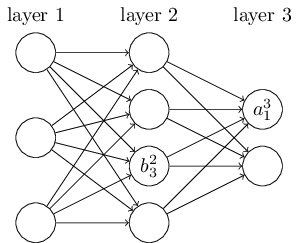
\includegraphics[width=0.5\textwidth]{./figs/tikz17.png}
\caption{Bias and activation notation}
\end{figure}

The activation $ a^l_j $ of the $ j^{th} $ neuron in the
$ l^{th} $ layer is related to the activations in the
$ (l - 1)^{th} $ layer by the equation

\begin{equation}
    a^l_j = \sigma(\sum_k w^l_{jk} a^{l-1}_k + b^l_j)
\end{equation}

where the sum is over all neurons $ k $ in the $ (l - 1)^{th} $
layer. Equation (18) can be rewritten in the beautiful and compact
vectorized form

\begin{equation}
    a^l = \sigma(w^l \cdot a^{l-1} + b^l)
\end{equation}

This expression gives us a much more global way of thinking about how
the activations in one layer relate to activations in the previous
layer: we just apply the weight matrix to the activations, then add the
bias vector, and finally apply the $ \sigma $ function. The expression is
also useful in practice, because most matrix libraries provide fast ways
of implementing matrix multiplication, vector addition, and
vectorization.

\subsection{2.2. The Hadamard product, $ s \odot t $}
\label{the-hadamard-product-s-t}

Suppose $ s $ and $ t $ are two vectors of the same dimension. Then
we use $ s \odot t $ to denote the elementwise product of the two
vectors. Thus the components of $ s \odot t $ are just $ {s \odot t}_j
= s_j t_j $. As an example,

\begin{equation}
    \left[ \begin{array}{c} 1 \\ 2 \end{array} \right] \odot
    \left[ \begin{array}{c} 3 \\ 4 \end{array} \right] = \left[
    \begin{array}{c} 1 \times 3 \\ 2 \times 4 \end{array} \right] =
    \left[ \begin{array}{c} 3 \\ 8 \end{array} \right]
\end{equation}

This kind of elementwise multiplication is sometimes called the Hadamard
product or Schur product. Good matrix libraries usually provide fast
implementations of the Hadamard product, and that comes in handy when
implementing backpropagation.

\subsection{2.3. The four fundamental equations behind backpropagation}
\label{the-four-fundamental-equations-behind-backpropagation}

We first introduce an intermediate quantity, $ \delta_j^l $,
which we call the error in the $ j^{th} $ neuron in the
$ l^{th} $ layer. Backpropagation will give us a procedure to
compute the error $ \delta_j^l $, and then will relate it to
$ \partial C / \partial w^l_{jk} $ and $ \partial C / \partial b^l_j $.

We define the error $ \delta^l_j $ of neuron $ j $ in layer
$ l $ by

\begin{equation}
    \delta^l_j \equiv \frac {\partial C}{\partial z^l_j}
\end{equation}

Backpropagation is based around four fundamental equations. Together,
those equations give us a way of computing both the error $ \delta^l $
and the gradient of the cost function.

An equation for the error in the output layer, $ \delta^L $:
The components of $ \delta^L $ are given by

\begin{equation}
    \delta^L_j = \frac {\partial C}{\partial a^L_j} \sigma^\prime
    (z^L_j)
\end{equation}

This is a very natural expression. The first term on the right,
$ \partial C / \partial a^L_j $,
just measures how fast the cost is changing as a function of the
$ j^{th} $ output activation. If, for example, $ C $ doesn't
depend much on a particular output neuron, $ j $, then $ \delta^L_j $
will be small, which is what we'd expect. The second term on the
right, $ \sigma^{\prime}z^L_j) $, measures how fast the activation function
$ \sigma $ is changing at $ z^L_j $. If we're using the quadratic cost function then
$ C = \frac{1}{2} \sum_j (y_j - a_j)^2 $, and so $ \partial C /
\partial a^L_j = (a_j - y_j) $, which obviously is easily computable.

It's easy to rewrite the Equation (22) in a matrix-based form, as

\begin{equation}
    \delta^L = (a^L - y) \odot \sigma^\prime (z^L)
\end{equation}

An equation for the error $ \delta^l $ in terms of the error in the
next layer, $ \delta_l + 1 $: In particular

\begin{equation}
    \delta^l = ((w^{l + 1})^T \delta^{l + 1}) \odot \sigma^\prime (z^l)
\end{equation}

We can think intuitively of this as moving the error backward through
the network, giving us some sort of measure of the error at the output
of the $ l^{th} $ layer.

By combining (23) with (24) we can compute the error $ \delta^l $ for
any layer in the network. We start by using (23) to compute
$ \delta^L $, then apply Equation (24) to compute $ \delta^{L - 1} $,
then $ \delta^{L - 2} $, and so on, all the way back through
the network.

An equation for the rate of change of the cost with respect to any bias
in the network: In particular:

\begin{equation}
    \frac {\partial C}{\partial b^l_j} = \delta^l_j
\end{equation}

or in shorthand as

\begin{equation}
    \frac {\partial C}{\partial b} = \delta
\end{equation}

where it is understood that $ \delta $ is being evaluated at the same
neuron as the bias $ b $.

An equation for the rate of change of the cost with respect to any
weight in the network: In particular:

\begin{equation}
    \frac {\partial C}{\partial w^l_{jk}} = a^{l - 1}_k\delta^l_j
\end{equation}

This tells us how to compute the partial derivatives $ \partial C /
\partial w^l_{jk} $ in terms of the quantities $ \delta^l $
and $ a^{l - 1} $, which we already know how to compute. The
equation can be rewritten in a less index-heavy notation as

\begin{equation}
    \frac {\partial C}{\partial w} = a_{in} \delta_{out}
\end{equation}

where it's understood that $ a_{in} $ is the activation of the
neuron input to the weight $ w $, and $ \delta_{out} $ is the error
of the neuron output from the weight $ w $.

A nice consequence of Equation (28) is that when the activation
$ a_{in} $ is small, $ a_{in} \approx 0 $, the gradient term
$ \partial C / \partial w $ will also tend to be small. In this case,
we'll say the weight learns slowly, meaning that it's not changing much
during gradient descent. In other words, one consequence of (28) is that
weights output from low-activation neurons learn slowly.

Recall from the graph of the sigmoid function in the last chapter that
the $ \sigma $ function becomes very flat when $ \sigma (z^L_j) $
is approximately 0 or 1. When this occurs we will have
$ \sigma^{\prime}(z^L_j) \approx 0 $.
And so the lesson is that a weight in the final layer will learn slowly
if the output neuron is either low activation $ (\approx 0) $
or high activation $ (\approx 1) $.

Summing up, we've learnt that a weight will learn slowly if either the
input neuron is low-activation, or if the output neuron has saturated,
i.e., is either high- or low-activation.

The four fundamental equations turn out to hold for any activation
function, not just the standard sigmoid function (that's because, the
proofs don't use any special properties of σ). And so we can use these
equations to design activation functions which have particular desired
learning properties. As an example to give you the idea, suppose we were
to choose a (non-sigmoid) activation function $ \sigma $ so that $
\sigma^{\prime} $ is always positive, and never gets close to zero.
That would prevent the slow-down of learning that occurs when ordinary
sigmoid neurons saturate.

\begin{figure}[htp]
\centering
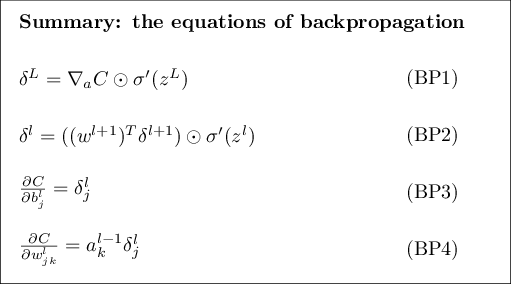
\includegraphics{./figs/tikz21.png}
\caption{Four fundamental equations of backpropapagation}
\end{figure}

The proof of four fundamental equations of backpropagation is just
coming from systematically applying the chain rule to the cost function
so that we may be able to get gradients of it.

\subsection{2.4. The backpropagation algorithm}
\label{the-backpropagation-algorithm}

The backpropagation equations provide us with a way of computing the
gradient of the cost function. Let's explicitly write this out in the
form of an algorithm:

\begin{enumerate}
\def\labelenumi{\arabic{enumi}.}
\item
  Input $ x $: Set the corresponding activation $ a^1 $ for the
  input layer.
\item
  Feedforward: For each $ l = 2, 3, \ldots{}, L $ compute $ z^l =
  w^l a^{l - 1} + b^l $ and $ a^l = \sigma (z^l) $.
\item
  Output error $ \delta^L $: Compute the vector $ \delta^L =
  \nabla_a C \odot \sigma^{\prime} (z^L) $.
\item
  Backpropagate the error: For each $ l = L - 1, L - 2, \ldots{}, 2 $
  compute $ \delta^l = ((w^{l + 1})^T \delta^{l +
  1}) \odot \sigma^{\prime} (z^l) $.
\item
  Output: The gradient of the cost function is given by
  $ \frac{\partial C}{\partial w^l_{jk}} = a^{l - 1}\sum_k
  \delta^l_j $ and $ \frac{\partial C}{\partial b^l_j} =
  \delta^l_j $.
\end{enumerate}

Examining the algorithm you can see why it's called backpropagation. We
compute the error vectors $ \delta^l $ backward, starting from the
final layer. The backward movement is a consequence of the fact that the
cost is a function of outputs from the network. To understand how the
cost varies with earlier weights and biases we need to repeatedly apply
the chain rule, working backward through the layers to obtain usable
expressions.

In practice, it's common to combine backpropagation with a learning
algorithm such as stochastic gradient descent, in which we compute the
gradient for many training examples. In particular, given a mini-batch
of $ m $ training examples, the following algorithm applies a gradient
descent learning step based on that mini-batch:

\begin{enumerate}
\def\labelenumi{\arabic{enumi}.}
\item
  Input a set of training examples
\item
  For each training example
  $ x $: Set the corresponding input activation $ a^{x, 1} $, and
  perform the following steps:
\item
  Feedforward: For each $ l = 2, 3, \ldots{}, L $ compute $ z^{x,
  l} = w^l a^{x,l - 1} + b^l $ and $ a^{x, l} =
  \sigma (z^{x, l}) $ .
\item
  Output error $ \delta^{x, L} $: Compute the vector $
  \delta^{x, L} = \nabla_a C_x
  \odot \sigma^{\prime} (z^{x, L}) $.
\item
  Backpropagate the error: For each $ l = L - 1, L - 2, \ldots{}, 2 $
  compute $ \delta^{x, l} = ((w^{l + 1})^T \delta^{x,
  l + 1}) \odot \sigma^{\prime} (z^{x, l}) $.
\item
  Gradient descent: For each $ l = L, L - 1, \ldots{}, 2 $ update the
  weights according to the rule $ w^l \to w^l -
  \frac{\eta}{m}\sum_x \delta^{x, l} (a^{x, l - 1})^T $,
  and the biases according to the rule $ b^l \to b^l -
  \frac{\eta}{m} \sum_x \delta^{x, l} $.
\end{enumerate}

Of course, to implement stochastic gradient descent in practice you also
need an outer loop generating mini-batches of training examples, and an
outer loop stepping through multiple epochs of training.

\section{3. Improving the way neural networks learn}
\label{improving-the-way-neural-networks-learn}

In this chapter it's explained a suite of techniques which can be used
to improve the implementation of backpropagation, and so improve the way
our networks learn.

The techniques we'll develop in this chapter include: a better choice of
cost function, known as the cross-entropy cost function; four
``regularization'' methods (L1 and L2 regularization, dropout, and
artificial expansion of the training data), which make our networks
better at generalizing beyond the training data; a better method for
initializing the weights in the network; and a set of heuristics to help
choose good hyper-parameters for the network.

\subsection{3.1. The cross-entropy cost function}
\label{the-cross-entropy-cost-function}

Ideally, we hope and expect that our neural networks will learn fast
from their errors. Is this what happens in practice? To answer this
question, let's look at a toy example. The example involves a neuron
with just one input:

\begin{figure}[htbp]
\centering
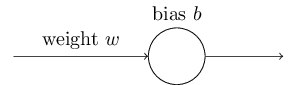
\includegraphics[width=0.5\textwidth]{./figs/tikz28.png}
\caption{Simple neuron}
\end{figure}

We'll train this neuron taking the input 1 to the output 0. Of course,
this is such a trivial task that we could easily figure out an
appropriate weight and bias by hand, without using a learning algorithm.
However, it turns out to be illuminating to use gradient descent to
attempt to learn a weight and bias. So let's take a look at how the
neuron learns.

To make things definite, we'll pick the initial weight to be 0.6 and the
initial bias to be 0.9 generically. The initial output from the neuron
is 0.82, so quite a bit of learning will be needed before our neuron
gets near the desired output, 0.0. The learning rate is $ \eta = 0.15. $
The cost is the quadratic cost function, $ C $. Code and the result
shown below.

\begin{verbatim}
import matplotlib.pylab as plt
import numpy as np

class Sigmoid(object):

    def activate(self, z):
        return 1. / (1. + np.exp(-z))

    def diff(self, z):
        return self.activate(z) * (1. - self.activate(z))

class QuadraticCost(object):

    def cost(self, y, out):
        return 0.5 * ((y - out)  2.)

    def diff(self, y, out):
        return (out - y)

class CrossEntropyCost(object):

    def cost(self, y, out):
        return -(y  np.log(out) + (1. - y) * np.log(1. - out))

    def diff(self, y, out):
        return (y - out) / (out * (out - 1.))

def singleNeuronModel(weight, bias, x=1.0, y=0.0, \
                      costFunction=QuadraticCost(),
                      eta=0.15, \
                      activationFunction=Sigmoid(), \
                      epoch=300):
'''
Models a single neuron for given weight and bias.
Input x = 1.0 and expected output y = 0.0.
Learning rate eta = 0.15.
Epoch (total training number) is 300.
'''
allCosts = []
for i in range(epoch):
    z = x  weight + bias
    out = activationFunction.activate(z)
    weight -= eta * costFunction.diff(y, out) * \
              activationFunction.diff(z) * out
    bias -= eta * costFunction.diff(y, out) * \
            activationFunction.diff(z)
    allCosts.append(costFunction.cost(y, out))

# Last out value with updated weights and biases.
z = x * weight + bias
out = activationFunction.activate(z)
allCosts.append(costFunction.cost(y, out))

# Print last weight, bias and output and drawing.
print "weight: {}, bias: {}, output: {}".format \
      (weight, bias, allCosts[-1])
plt.plot(range(epoch + 1), allCosts)
plt.xlabel('epochs')
plt.ylabel('cost')
plt.show()

-----

singleNeuronModel(weight=0.6, bias=0.9)
\end{verbatim}

\begin{figure}[htp]
\centering
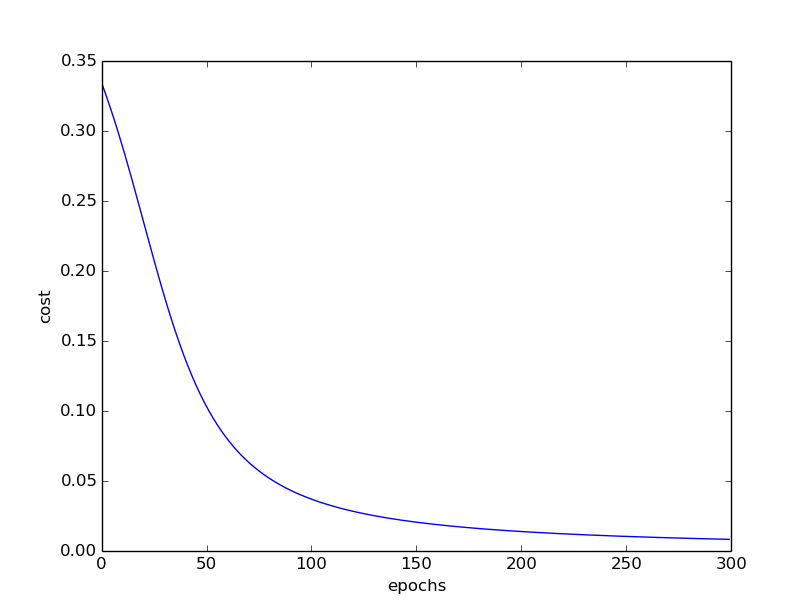
\includegraphics[width=0.7\textwidth]{./figs/single_neuron1.png}
\caption{Single neuron with weight=0.6, bias=0.9}
\end{figure}

As you can see, the neuron rapidly learns a weight and bias that drives
down the cost, and gives an output 0.008. Suppose, however, that we
instead choose both the starting weight and the starting bias to be 2.0.
In this case the initial output is 0.98, which is very badly wrong.
Let's look at how the neuron learns to output 0 in this case.

\begin{verbatim}
singleNeuronModel(weight=2.0, bias=2.0)
\end{verbatim}

\begin{figure}[htp]
\centering
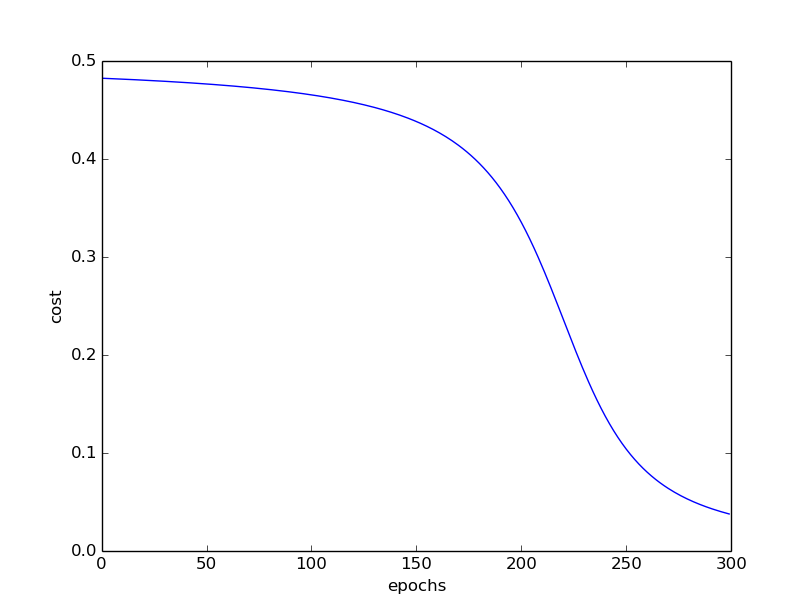
\includegraphics[width=0.7\textwidth]{./figs/single_neuron3.png}
\caption{Single neuron with weight=2.0, bias=2.0}
\end{figure}

Although this example uses the same learning rate $ (\eta = 0.15) $,
we can see that learning starts out much more slowly. Indeed, for the
first 150 or so learning epochs, the weights and biases don't change
much at all.


This behaviour is strange when contrasted to human learning. As I said
at the beginning of this section, we often learn fastest when we're
badly wrong about something. But we've just seen that our artificial
neuron has a lot of difficulty learning when it's badly wrong - far more
difficulty than when it's just a little wrong. What's more, it turns out
that this behaviour occurs not just in this toy model, but in more
general networks. Why is learning so slow? And can we find a way of
avoiding this slowdown?

To understand the origin of the problem, let's compute the partial
derivatives. Recall that we're using the quadratic cost function,

\begin{equation}
    C = \frac {(y - a)^2}{2}
\end{equation}

where $ a $ is the neuron's output when the training input $ x = 1 $
is used, and $ y = 0 $ is the corresponding desired output. Recall
that $ a = \sigma(z) $, where $ z = w \cdot x + b $. Using the chain rule to
differentiate with respect to the weight and bias we get

\begin{equation}
    \begin{split}
        \frac {\partial C}{\partial w} &= \frac {\partial C}{\partial a}
        \frac {\partial a}{\partial \sigma} \frac {\partial \sigma}{\partial w} =
        (a - y) \sigma^\prime(z) x = a \sigma^\prime(z) \\
        \frac {\partial C}{\partial b} &= \frac {\partial C}{\partial a}
        \frac {\partial a}{\partial \sigma} \frac {\partial \sigma}{\partial b} =
        (a - y) \sigma^\prime(z) =
        a \sigma^\prime(z)
    \end{split}
\end{equation}

where substituted $ x = 1 $ and $ y = 0
$. To understand the behaviour of these expressions, let's look more closely at the $
\sigma^{\prime} (z) $ term on the right-hand side. Recall the shape of
the $ \sigma $ function:

\begin{figure}[htp]
\centering
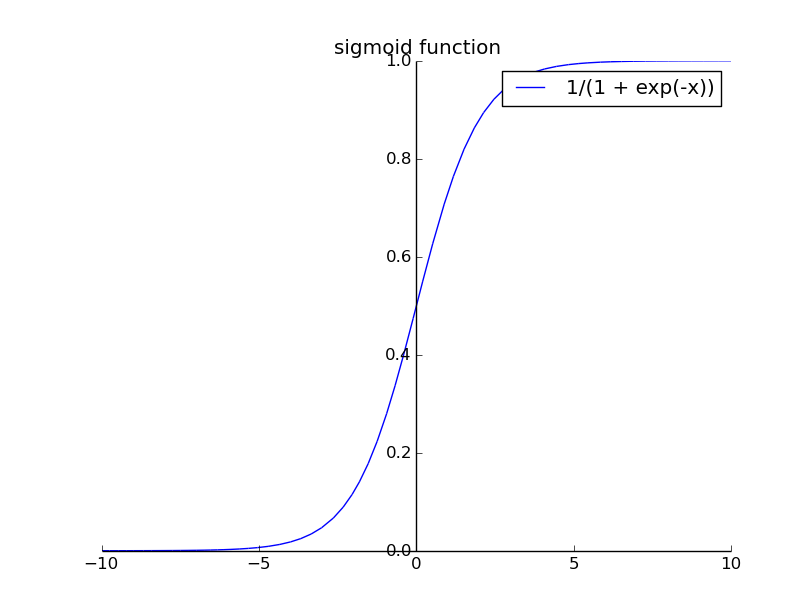
\includegraphics[width=0.7\textwidth]{./figs/sigmoid_function.png}
\caption{Sigmoid function}
\end{figure}

We can see from this graph that when the neuron's output is close to 1,
the curve gets very flat, and so $ \sigma^{\prime} (z) $ gets very
small. Therefore $ \partial C / \partial w $ and $ \partial C /
\partial b $ get very small. This is the origin of the learning
slowdown.

\subsection{3.2. Introducing the cross-entropy cost function}
\label{introducing-the-cross-entropy-cost-function}

How can we address the learning slowdown? It turns out that we can solve
the problem by replacing the quadratic cost with a different cost
function, known as the cross-entropy. To understand the cross-entropy,
let's move a little away from our super-simple toy model. We'll suppose
instead that we're trying to train a neuron with several input
variables, $ x_1, x_2, \ldots{} $ corresponding weights $ w_1,
w_2, \ldots{} $ and a bias, $ b $:

\begin{figure}[htp]
\centering
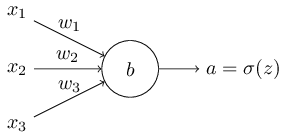
\includegraphics[width=0.5\textwidth]{./figs/tikz29.png}
\caption{A neuron with multiple inputs}
\end{figure}

The output from the neuron is, of course, $ a = \sigma(z) $, where $ z
= \sum_j w_j x_j + b $ is the weighted sum of the inputs. We
define the cross-entropy cost function for this neuron by

\begin{equation}
    C = -\frac{1}{n} \sum_x [y \ln a + (1 - y) \ln (1 - a)]
\end{equation}

where $ n $ is the total number of items of training data, the sum is
over all training inputs, $ x $, and $ y $ is the corresponding
desired output. The quantity $ -{[}y \ln a + (1 - y) \ln (1 - a){]} $
is sometimes known as the binary entropy.

Two properties in particular make it reasonable to interpret the
cross-entropy as a cost function. First, it's non-negative, that is, $
C \textgreater{} 0 $. $ y $ takes only $ 0 $ or $ 1 $ and $ a $
takes values between $ 0 $ and $ 1 $. Then $ \ln(1 - a) \textless{} 0
$ and $ \ln(a) \textless{} 0 $. The minus sign out of front provides $
C \textgreater{} 0 $.

Second, if the neuron's actual output is close to the desired output,
i.e., $ y = y(x) $ for all training inputs $ x $ , then the
cross-entropy will be close to zero.

\begin{verbatim}
>>> import sympy as sp
>>> a, y = sp.symbols("a y")
>>> expr = - (y  sp.ln(a) + (1 - y)  sp.ln(1 - a))
>>> expr.subs({y:0, a:0.00001})
    1.00000500002878e-5
>>> expr.subs({y:1, a:0.99999})
    1.00000500005137e-5
\end{verbatim}

To see this, let's compute the partial derivative of the cross-entropy
cost with respect to the weights. We substitute $ a = \sigma(z) $ into
(31), and apply the chain rule twice, obtaining:

\begin{equation}
    \begin{split}
        \frac{\partial C}{\partial w_j} & = -\frac{1}{n}\sum_x \left (
        \frac{y}{\sigma(z)} - \frac{(1 - y)}{1 - \sigma(z)} \right)
        \frac{\partial \sigma}{\partial w_j} \\
        & = -\frac{1}{n}\sum_x \left (
        \frac{y}{\sigma(z)} - \frac{(1 - y)}{1 - \sigma(z)} \right)
        \sigma^{\prime} (z) x_j \\
        & = \frac{1}{n} \sum_x  \frac{\sigma ^ \prime(z) x_j}
        {\sigma(z)[1 - \sigma(z)]}(\sigma(z) - y)
     \end{split}
\end{equation}

We know that $ \sigma^{\prime}(z) = \sigma(z){[}1 - \sigma(z){]} $.
Therefore (32) becomes,

\begin{equation}
    \frac{\partial C}{\partial w_j} = \frac{1}{n} \sum_x x_j [\sigma(z) - y]
\end{equation}

This is a beautiful expression. It tells us that the larger the error,
the faster the neuron will learn. In a similar way, it can be easily
verified that

\begin{equation}
    \frac{\partial C}{\partial b} = \frac{1}{n} \sum_x [\sigma(z) - y]
\end{equation}

Let's return to the toy example we played with earlier, and explore what
happens when we use the cross-entropy instead of the quadratic cost. To
re-orient ourselves, we'll begin with the case where the quadratic cost
did just fine, with starting weight 0.6 and starting bias 0.9.

\begin{verbatim}
singleNeuronModel(weight=0.6, bias=0.9, \
                  costFunction=CrossEntropyCost())
\end{verbatim}

\begin{figure}[htp]
\centering
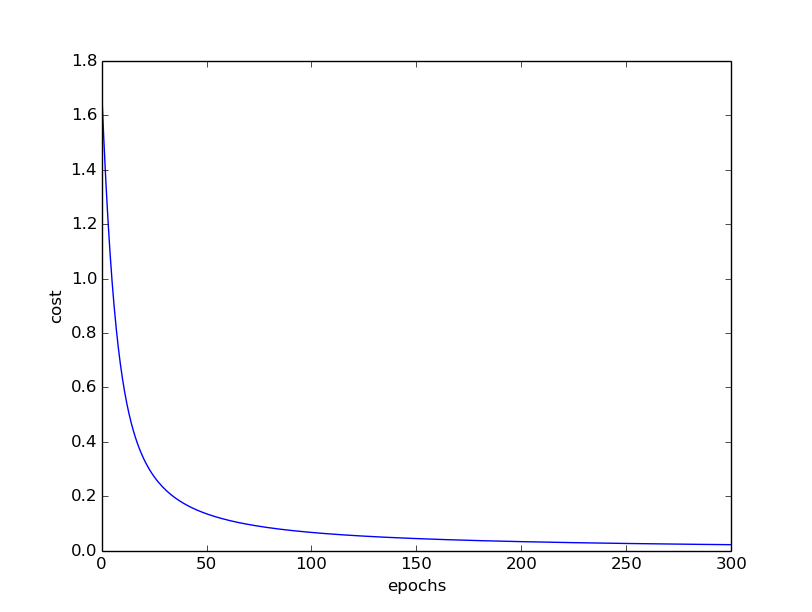
\includegraphics[width=0.7\textwidth]{./figs/single_neuron2_cross_entropy_cost.png}
\caption{Single neuron with cross entropy cost with weight=0.6, bias=0.9}
\end{figure}

Now with starting weight 2.0 and starting bias 2.0.

\begin{verbatim}
singleNeuronModel(weight=2.0, bias=2.0, \
                  costFunction=CrossEntropyCost())
\end{verbatim}

\begin{figure}[htp]
\centering
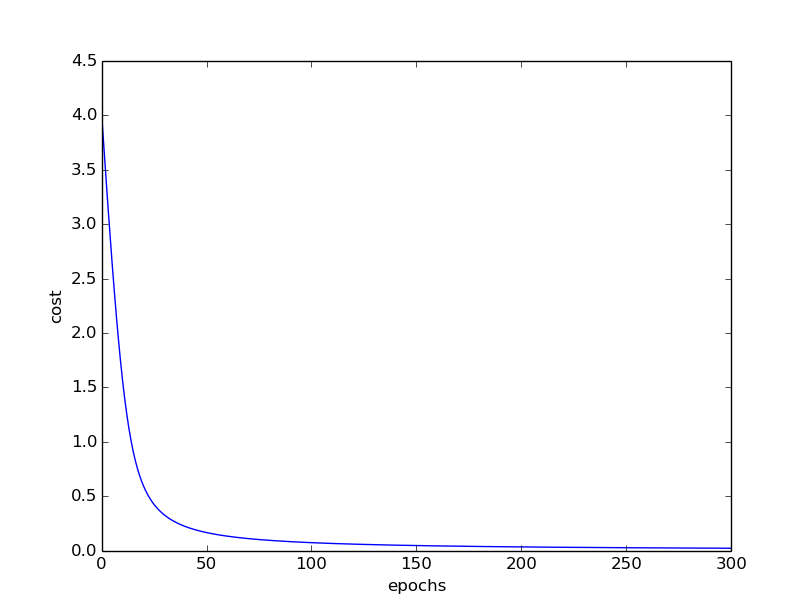
\includegraphics[width=0.7\textwidth]{./figs/single_neuron4_cross_entropy_cost.png}
\caption{Single neuron with cross entropy cost with weight=2.0, bias=2.0}
\end{figure}

Success! This time the neuron learned quickly, just as we hoped.

We've been studying the cross-entropy for a single neuron. However, it's
easy to generalize the cross-entropy to many-neuron multi-layer
networks. In particular, suppose $ y = y_1, y_2, \ldots{} $ are the
desired values at the output neurons, i.e., the neurons in the final
layer, while $ a^L_1, a^L_2, \ldots{} $are the actual output
values. Then we define the cross-entropy by

\begin{equation}
        C = -\frac{1}{n} \sum_x \sum_j \left[ y_j \ln a^L_j +
        (1 - y_j) \ln (1 - a^L_j) \right ]
\end{equation}

When should we use the cross-entropy instead of the quadratic cost? In
fact, the cross-entropy is nearly always the better choice, provided the
output neurons are sigmoid neurons. To see why, consider that when we're
setting up the network we usually initialize the weights and biases
using some sort of randomization. It may happen that those initial
choices result in the network being decisively wrong for some training
input - that is, an output neuron will have saturated near 1, when it
should be 0, or vice versa. If we're using the quadratic cost that will
slow down learning.

\subsection{3.3. Softmax}\label{softmax}

The idea of softmax is to define a new type of output layer for our
neural networks. It begins in the same way as with a sigmoid layer, by
forming the weighted inputs as $ z^L_j = \sum_k w^L_{jk}
a^{L - 1}\sum_k + b^L_j $.
However, in a softmax layer we apply the so-called softmax function to the
$ z^L_j $. According to this function, the activation $ a^L_j $
of the $ j^{th} $ output neuron is

\begin{equation}
    a^L_j = \frac{e^{z^L_j}}{\sum_k e^{z^L_k}}
\end{equation}

where in the denominator we sum over all the output neurons.

To better understand Equation (36), suppose we have a network with four
output neurons, and four corresponding weighted inputs, which we'll
denote $ z^L_1, z^L_2, z^L_3 $ and $ z^L_4 $. As you increase $ z^L_4 $,
you'll see an increase in the corresponding output activation, $ a^L_4 $,
and a decrease in the other output activations. Similarly, if you decrease
$ z^L_4 $ then $ a^L_4 $ will decrease, and all the other
output activations will increase. In fact, if you look closely, you'll
see that in both cases the total change in the other activations exactly
compensates for the change in $ a^L_4 $. The reason is that the output
activations are guaranteed to always sum up to $ 1 $,

\begin{equation}
        \sum_j a^L_j = \frac{\sum_j e^{z^L_j}}{\sum_k e^{z^L_k}} = 1
\end{equation}

And, of course, similar statements hold for all the other activations.

Equation (37) implies that the output from the softmax layer is a set of
positive numbers which sum up to 1. In other words, the output from the
softmax layer can be thought of as a probability distribution.

In many problems it's convenient to be able to interpret the output
activation $ a^L_j $ as the network's estimate of the probability
that the correct output is $ j $. So, for instance, in the
MNIST classification problem, we can interpret
$ a^L_j $ as the network's estimated probability that the correct
digit classification is $ j $.

The learning slowdown problem: How a softmax layer lets us address the
learning slowdown problem? To understand that, let's define the
log-likelihood cost function. We'll use $ x $ to denote a training
input to the network, and $ y $ to denote the corresponding desired
output. Then the log-likelihood cost associated to this training input
is

\begin{equation}
    C \equiv −\ln a^L_y
\end{equation}

So, for instance, if we're training with MNIST images, and input an
image of a 7, then the log-likelihood cost is $ −\ln a^L_7 $.
To see that this makes intuitive sense, consider the case when the network
is doing a good job, that is, it is confident the input is a $ 7 $.
In that case it will estimate a value for the corresponding probability
$ a^L_7 $ which is close to $ 1 $, and so the cost $ −\ln a^L_7 $ will be small.
By contrast, when the network isn't doing such a good
job, the probability $ a^L_7 $ will be smaller, and the cost
$ −\ln a^L_7 $ will be larger. Unlike quadratic cost function and
cross-entropy function, no need to sum all the cost in the output
neurons, only corresponding neuron must be considered. Because the cost
of output neurons are related each other to make $ \sum_j a^L_j = 1 $.

What about the learning slowdown problem? With a little algebra you can
show that.

\begin{equation}
    \begin{split}
        \frac{\partial C}{\partial b^L_j} & = a^L_j - y_j \\
        \frac{\partial C}{\partial w^L_{jk}} & = a^{L - 1}_k(a^L_j - y_j)
    \end{split}
\end{equation}

Here we used $ y $ to denote the desired output from the network -
e.g., output a ``$ 7 $" if an image of a $ 7 $ was input. But in the
equations here $ y $ to denote the vector of output activations which
corresponds to $ 7 $, that is, a vector which is all $ 0 $ s, except
for a $ 1 $ in the $ 7^{th} $ location.

Just as in the earlier analysis, these expressions ensure that we will
not encounter a learning slowdown. In fact, it's useful to think of a
softmax output layer with log-likelihood cost as being quite similar to
a sigmoid output layer with cross-entropy cost.

\subsection{3.4. Overfitting}\label{overfitting}

Overfitting is a major problem in neural networks. This is especially
true in modern networks, which often have very large numbers of weights
and biases.

Let's sharpen this problem up by constructing a situation where our
network does a bad job generalizing to new situations. We'll use our 30
hidden neuron network, with its 23,860 parameters. But we won't train
the network using all 50,000 MNIST training images. Instead, we'll use
just the first 1,000 training images. Using that restricted set will
make the problem with generalization much more evident. We'll train in a
similar way to before, using the cross-entropy cost function, with a
learning rate of $ \eta = 0.5 $ and a mini-batch size of 10. However,
we'll train for 400 epochs, a somewhat larger number than before,
because we're not using as many training examples. Get network2.py
from https://github.com/mnielsen/neural-networks-and-deep-learning
to look at the way the cost function changes:

\begin{verbatim}
>>> import mnist_loader
>>> training_data, validation_data, test_data = \
mnist_loader.load_data_wrapper()
>>> import network2
>>> net = network2.Network([784, 30, 10], \
                           cost=network2.CrossEntropyCost)
>>> net.large_weight_initializer()
>>> net.SGD(training_data[:1000], 400, 10, 0.5, \
evaluation_data=test_data, \
monitor_evaluation_accuracy=True, \
monitor_training_cost=True)
\end{verbatim}

Using the results we can plot the way the cost changes as the network
learns.

\begin{figure}[htp]
\centering
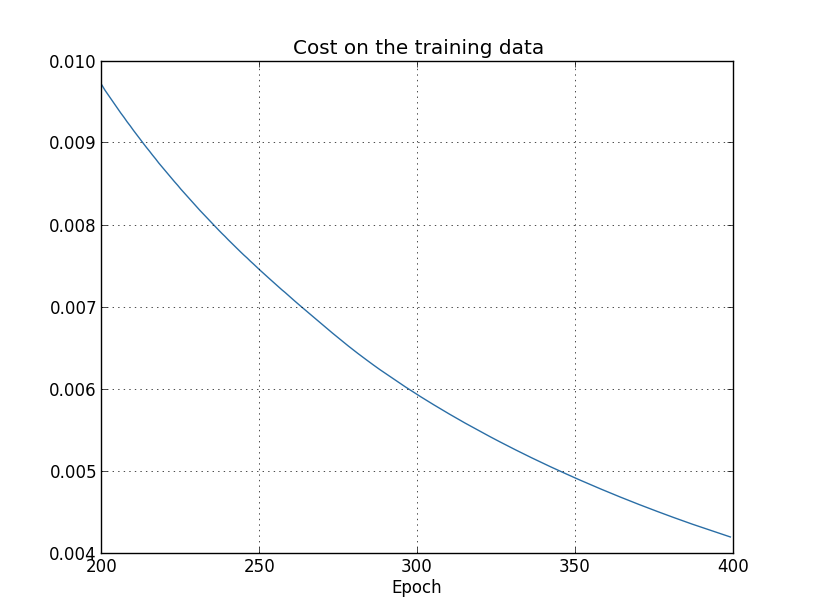
\includegraphics[width=0.7\textwidth]{./figs/overfitting1.png}
\caption{Overfitting effect on the cost of training data}
\end{figure}

This looks encouraging, showing a smooth decrease in the cost, just as
we expect. Let's now look at how the classification accuracy on the test
data changes over time:

\begin{figure}[htp]
\centering
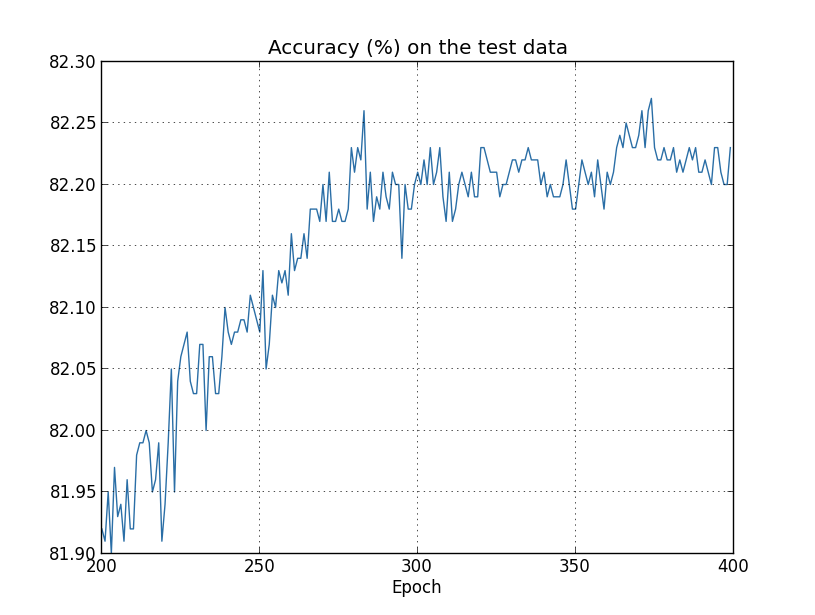
\includegraphics[width=0.7\textwidth]{./figs/overfitting2.png}
\caption{Overfitting effect on the accuracy of test data}
\end{figure}

If we just look at that cost, it appears that our model is still getting
``better''. But the test accuracy results show the improvement is an
illusion. What our network learns after epoch 280 no longer generalizes
to the test data. And so it's not useful learning. We say the network is
overfitting or overtraining beyond epoch 280.

Another sign of overfitting may be seen in the classification accuracy
on the training data:

\begin{figure}[htp]
\centering
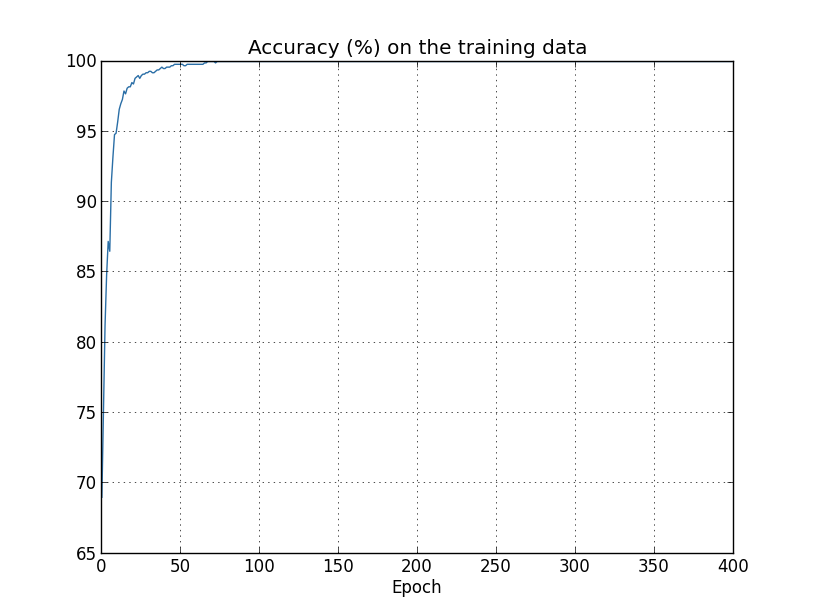
\includegraphics[width=0.7\textwidth]{./figs/overfitting4.png}
\caption{Overfitting effect on the accuracy of training data}
\end{figure}

The accuracy rises all the way up to 100 percent. That is, our network
correctly classifies all 1,000 training images! Meanwhile, our test
accuracy tops out at just 82.27 percent. So our network really is
learning about peculiarities of the training set, not just recognizing
digits in general. It's almost as though our network is merely
memorizing the training set, without understanding digits well enough to
generalize to the test set.

The obvious way to detect overfitting is to use the approach above,
keeping track of accuracy on the test data as our network trains. If we
see that the accuracy on the test data is no longer improving, then we
should stop training. Of course, strictly speaking, this is not
necessarily a sign of overfitting. It might be that accuracy on the test
data and the training data both stop improving at the same time. Still,
adopting this strategy will prevent overfitting.

In fact, we'll use a variation on this strategy. Recall that when we
load in the MNIST data we load in three data sets:

\begin{verbatim}
>>> import mnist_loader
>>> training_data, validation_data, test_data = \
mnist_loader.load_data_wrapper()
\end{verbatim}

Up to now we've been using the `training data' and `test data', and
ignoring the `validation data'. The `validation data' contains 10,000
images of digits, images which are different from the 50,000 images in
the MNIST training set, and the 10,000 images in the MNIST test set.

Instead of using the `test data' to prevent overfitting, we will use
the `validation data'. To do this, we'll use much the same strategy as
was described above for the `test data'. That is, we'll compute the
classification accuracy on the `validation data' at the end of each
epoch. Once the classification accuracy on the `validation data' has
saturated, we stop training. This strategy is called early stopping. Of
course, in practice we won't immediately know when the accuracy has
saturated. Instead, we continue training until we're confident that the
accuracy has saturated. It requires some judgement to determine when to
stop.

You can think of the validation data as a type of training data that
helps us learn good hyper-parameters. This approach to finding good
hyper-parameters is sometimes known as the hold out method, since the
`validation data' is kept apart from the `training data'.

What happens when we use the full training set of 50,000 images? Here's
a graph showing the results for the classification accuracy on both the
training data and the test data.

\begin{figure}[htp]
\centering
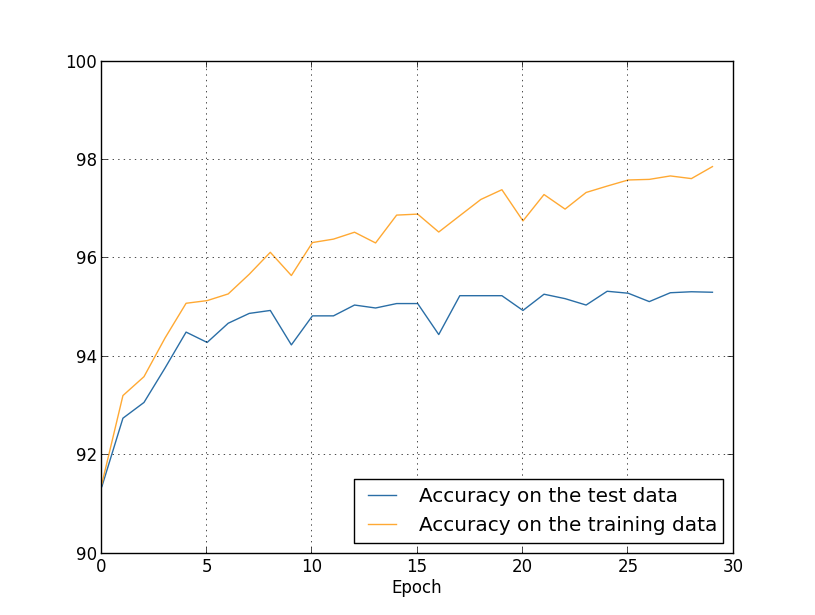
\includegraphics[width=0.7\textwidth]{./figs/overfitting_full.png}
\caption{Comparison of accuracies in training and test data}
\end{figure}

As you can see, the accuracy on the test and training data remain much
closer together than when we were using 1,000 training examples.
Overfitting is still going on, but it's been greatly reduced. Our
network is generalizing much better from the training data to the test
data. In general, one of the best ways of reducing overfitting is to
increase the size of the training data. Unfortunately, training data can
be expensive or difficult to acquire, so this is not always a practical
option.

\subsection{3.5. Regularization}\label{regularization}

Fortunately, there are other techniques which can reduce overfitting,
even when we have a fixed network and fixed training data. These are
known as regularization techniques. One of the most commonly used
regularization techniques are weight decay or L2 regularization. The
idea of L2 regularization is to add an extra term to the cost function,
a term called the regularization term. Here's the regularized
cross-entropy:

\begin{equation}
    C = -\frac{1}{n} \sum_{xj} \left [
    y_j \ln a^L_j + (1 - y_j) \ln (1 - a^L_j) \right ] +
    \frac{\lambda}{2n} \sum_w w^2
\end{equation}

The first term is just the usual expression for the cross-entropy. But
we've added a second term, namely the sum of the squares of all the
weights in the network. This is scaled by a factor $ \lambda / 2n $,
where $ \lambda \textgreater{} 0 $ is known as the regularization
parameter, and $ n $ is, as usual, the size of our training set.

Of course, it's possible to regularize other cost functions, such as the
quadratic cost. This can be done in a similar way:

\begin{equation}
    C = -\frac{1}{2n} \sum_x || y - a^L ||^2 +
    \frac{\lambda}{2n} \sum_w w^2
\end{equation}

Intuitively, the effect of regularization is to make it so the network
prefers to learn small weights, all other things being equal. Large
weights will only be allowed if they considerably improve the first part
of the cost function. Regularization can be viewed as a way of
compromising between finding small weights and minimizing the original
cost function. When $ \lambda $ is small we prefer to minimize the
original cost function, but when $ \lambda $ is large we prefer small
weights.

To construct such an example, we first need to figure out how to apply
our stochastic gradient descent learning algorithm in a regularized
neural network. In particular, we need to know how to compute the
partial derivatives $ \partial C / \partial w $ and $ \partial C /
\partial b $ for all the weights and biases in the network.

\begin{equation}
    \begin{split}
        \frac{\partial C}{\partial w} & = \frac{\partial C_0}{\partial w} +
        \frac{\lambda}{n} w \\
        \frac{\partial C}{\partial b} & = \frac{\partial C_0}{\partial b}
    \end{split}
\end{equation}

The $ \partial C_0 / \partial w $ and $ \partial C_0 / \partial b $
terms can be computed using backpropagation. Then add
$ \frac{\lambda}{n} w $ to the partial derivative of all the weight
terms. The partial derivatives with respect to the biases are unchanged,
and so the gradient descent learning rule for the biases doesn't change
from the usual rule:

\begin{equation}
    b \to b − \eta \frac{\partial C_0}{\partial b}
\end{equation}

The learning rule for the weights becomes:

\begin{equation}
    \begin{split}
        w & \to w − \eta \frac{\partial C_0}{\partial w} -
        \frac{\eta \lambda}{n} w \\
        &= \left (1 - \frac{\eta \lambda}{n} \right ) w - \eta
        \frac{\partial C_0}{\partial w}
    \end{split}
\end{equation}

This is exactly the same as the usual gradient descent learning rule,
except we first rescale the weight $ w $ by a factor $ 1 - \frac{\eta \lambda}{n} $.
This rescaling is sometimes referred to as
weight decay, since it makes the weights smaller. At first glance it
looks as though this means the weights are being driven unstoppably
toward zero. But that's not right, since the other term may lead the
weights to increase.

For stochastic gradient descent Equation (43) becomes

\begin{equation}
    b \to b - \frac{\eta}{m} \sum_x \frac{\partial C_x}{\partial b}
\end{equation}

Equation (44) becomes

\begin{equation}
    w \to \left (1 - \frac{\eta \lambda}{n} \right ) w -
    \frac{\eta}{m} \sum_x \frac{\partial C_x}{\partial w}
\end{equation}

where the sum is over training examples $ x $ in the mini-batch, and
$ C_x $ is the (unregularized) cost for each training example. And

Let's see how regularization changes the performance of our neural
network. We'll use a network with 30 hidden neurons, a mini-batch size
of 10, a learning rate of 0.5, and the cross-entropy cost function.
However, this time we'll use a regularization parameter of $ \lambda =
0.1 $.

\begin{verbatim}
>>> import mnist_loader
>>> training_data, validation_data, test_data =
mnist_loader.load_data_wrapper()
>>> import network2
>>> net = network2.Network([784, 30, 10],
cost=network2.CrossEntropyCost)
>>> net.large_weight_initializer()
>>> net.SGD(training_data[:1000], 400, 10, 0.5,
evaluation_data=test_data, lmbda = 0.1,
monitor_evaluation_cost=True,
monitor_evaluation_accuracy=True,
monitor_training_cost=True,
monitor_training_accuracy=True)
\end{verbatim}

The cost on the training data decreases over the whole time, much as it
did in the earlier, unregularized case.

\begin{figure}[htp]
\centering
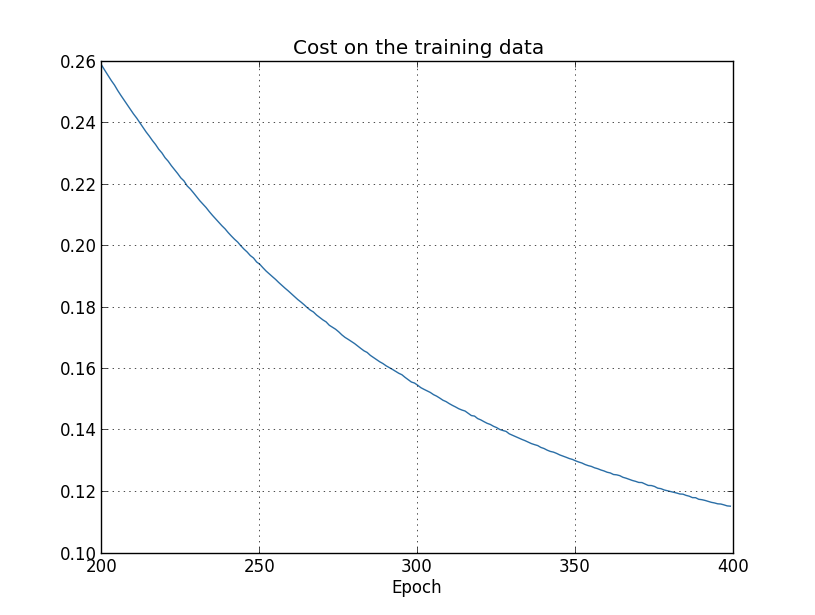
\includegraphics[width=0.7\textwidth]{./figs/regularized1.png}
\caption{Cost in training data for regularized case}
\end{figure}

But this time the accuracy on the `test data' continues to increase for
the entire 400 epochs:

\begin{figure}[htp]
\centering
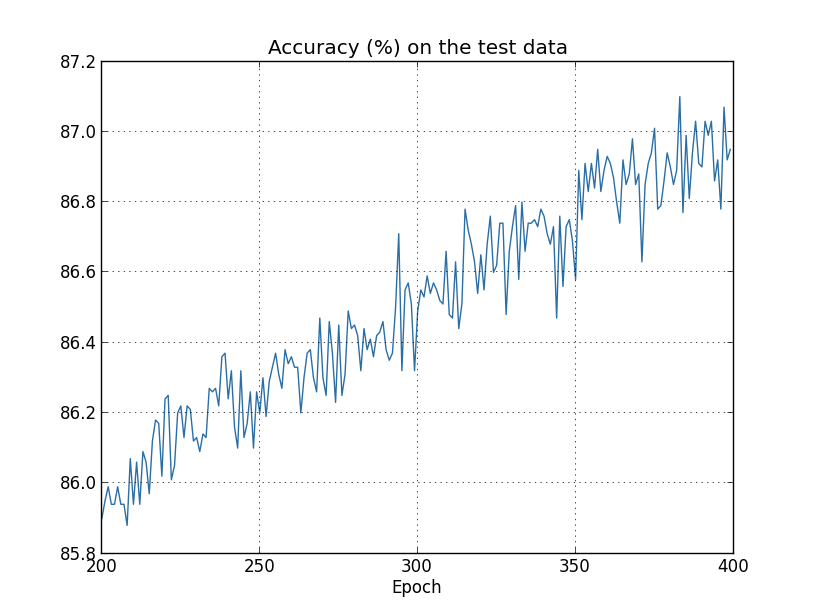
\includegraphics[width=0.7\textwidth]{./figs/regularized2.png}
\caption{Accuracy in test data for regularized case}
\end{figure}

Clearly, the use of regularization has suppressed overfitting. What's
more, the accuracy is considerably higher, with a peak classification
accuracy of $ 87.1 $ percent, compared to the peak of $ 82.27 $
percent obtained in the unregularized case. It seems that, empirically,
regularization is causing our network to generalize better, and
considerably reducing the effects of overfitting.

Let' train our network with full 50,000 images. The hyper-parameters the
same as before - 30 epochs, learning rate 0.5, mini-batch size of 10.
However, we need to modify the regularization parameter. The reason is
because the size $ n $ of the training set has changed from $ n =
1,000 $ to $ n = 50,000 $. If we continued to use $ \lambda = 0.1 $
that would mean much less weight decay, and thus much less of a
regularization effect. We compensate by changing to $ \lambda = 5.0 $.

\begin{verbatim}
>>> net.large_weight_initializer()
>>> net.SGD(training_data, 30, 10, 0.5,
evaluation_data=test_data, lmbda = 5.0,
monitor_evaluation_accuracy=True,
monitor_training_accuracy=True)
\end{verbatim}

\begin{figure}[htp]
\centering
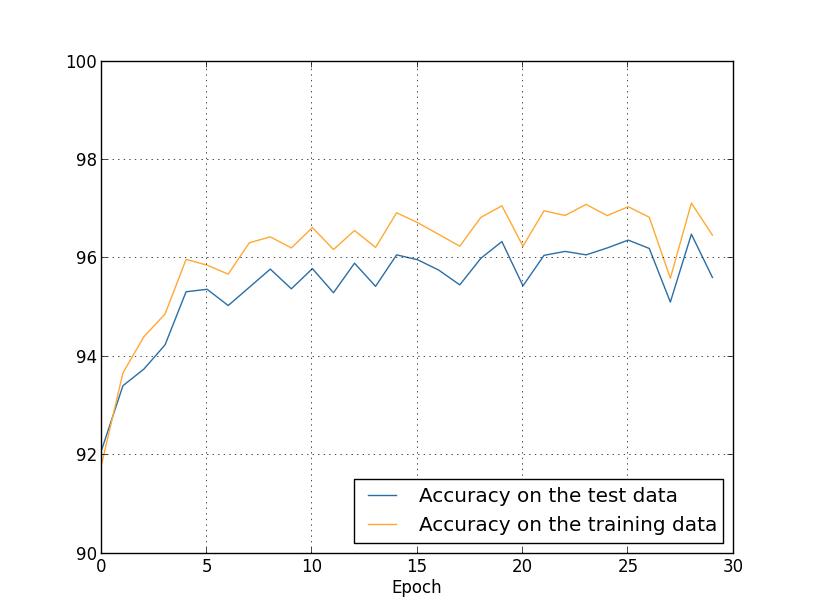
\includegraphics[width=0.7\textwidth]{./figs/regularized_full.png}
\caption{Comparison of accuracies of training and test data}
\end{figure}

There's lots of good news here. First, our classification accuracy on
the test data is up, from $ 95.49 $ percent when running
unregularized, to $ 96.49 $ percent. That's a big improvement. Second,
we can see that the gap between results on the training and test data is
much narrower than before, running at under a percent. That's still a
significant gap, but we've obviously made substantial progress reducing
overfitting.

Finally, let's see what test classification accuracy we get when we use
100 hidden neurons and a regularization parameter of $ \lambda = 5.0
$.

\begin{verbatim}
>>> net = network2.Network([784, 100, 10],
cost=network2.CrossEntropyCost)
>>> net.large_weight_initializer()
>>> net.SGD(training_data, 30, 10, 0.5, lmbda=5.0,
evaluation_data=validation_data,
monitor_evaluation_accuracy=True)
\end{verbatim}

The final result is a classification accuracy of $ 97.92 $ percent on
the validation data.

Empirically, when doing multiple runs of our MNIST networks, but with
different (random) weight initializations, I've found that the
unregularized runs will occasionally get ``stuck'', apparently caught in
local minima of the cost function. By contrast, the regularized runs
have provided much more easily replicable results.

Heuristically, if the cost function is unregularized, then the length of
the weight vector is likely to grow, all other things being equal. Over
time this can lead to the weight vector being very large indeed and can
cause the weight vector to get stuck pointing in more or less the same
direction, since changes due to gradient descent only make tiny changes
to the direction.

\subsection{3.5.1. Other techniques for regularization}
\label{other-techniques-for-regularization}

There are three other approaches to reducing overfitting: L1
regularization, dropout, and artificially expanding the training set
size.

\subsubsection{3.5.1.1. L1 regularization}\label{l1-regularization}

In this approach we modify the unregularized cost function by adding the
sum of the absolute values of the weights:

\begin{equation}
    C = C_0 + \frac{\lambda}{n} \sum_w |w|
\end{equation}

Intuitively, this is similar to L2 regularization, penalizing large
weights, and tending to make the network prefer small weights.

To do that, we'll look at the partial derivatives of the cost function.
Differentiating (47) we obtain:

\newcommand{\sgn}{\mathop{\mathrm{sgn}}}
\begin{equation}
    \frac{\partial C}{\partial w} = \frac{\partial C_0}{\partial w} +
    \frac{\lambda}{n} \sgn(w)
\end{equation}

where $ \sgn(w) $ is the sign of $ w $, that is, +1 if $ w $ is
positive, and −1 if $ w $ is negative. The resulting update rule for
an L1 regularized network is

\begin{equation}
    w\to w − \frac{\eta \lambda}{n} \sgn(w) -
    \eta \frac{\partial C_0}{\partial w}
\end{equation}

In both expressions the effect of regularization is to shrink the
weights. This accords with our intuition that both kinds of
regularization penalize large weights. But the way the weights shrink is
different. In L1 regularization, the weights shrink by a constant amount
toward 0. In L2 regularization, the weights shrink by an amount which is
proportional to w. And so when a particular weight has a large
magnitude, $ |w| $, L1 regularization shrinks the weight much less than
L2 regularization does. By contrast, when $ |w| $ is small, L1
regularization shrinks the weight much more than L2 regularization.
The net result is that L1 regularization tends to concentrate the
weight of the network in a relatively small number of high-importance connections,
while the other weights are driven toward zero.

Partial derivative $ \partial C / \partial w $ isn't defined when $ w
= 0 $. The reason is that the function $ |w| $ has a
sharp ``corner'' at $ w = 0 $, and so isn't differentiable at that point.
That's okay, though. We'll use Equations (48) and (49) with the convention that
$ \sgn(0) = 0 $.

\subsubsection{3.5.1.2. Dropout}\label{dropout}

Dropout is a radically different technique for regularization. In
dropout we modify the network itself. Suppose we're trying to train a
network:

\begin{figure}[htp]
\centering
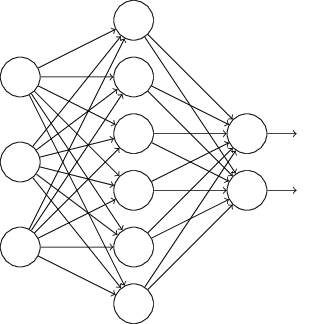
\includegraphics[width=0.5\textwidth]{./figs/tikz30.png}
\caption{MLP}
\end{figure}

With dropout, we start by randomly (and temporarily) deleting half the
hidden neurons in the network, while leaving the input and output
neurons untouched. After doing this, we'll end up with a network along
the following lines.

\begin{figure}[htp]
\centering
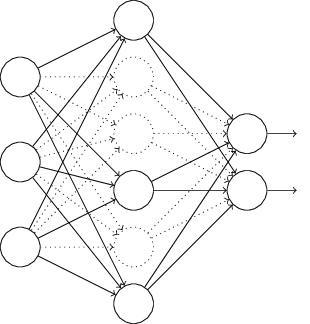
\includegraphics[width=0.5\textwidth]{./figs/tikz31.png}
\caption{Dropping neurons out}
\end{figure}

After doing this over a mini-batch of examples, we update the
appropriate weights and biases. We then repeat the process, first
restoring the dropout neurons, then choosing a new random subset of
hidden neurons to delete, estimating the gradient for a different
mini-batch, and updating the weights and biases in the network.

By repeating this process over and over, our network will learn a set of
weights and biases. Of course, those weights and biases will have been
learnt under conditions in which half the hidden neurons were dropped
out. When we actually run the full network that means that twice as many
hidden neurons will be active. To compensate for that, we halve the
weights outgoing from the hidden neurons.

Heuristically, when we dropout different sets of neurons, it's rather
like we're training different neural networks. And so the dropout
procedure is like averaging the effects of a very large number of
different networks. The different networks will overfit in different
ways, and so, hopefully, the net effect of dropout will be to reduce
overfitting.

In other words, if we think of our network as a model which is making
predictions, then we can think of dropout as a way of making sure that
the model is robust to the loss of any individual piece of evidence.

Here some dropout results applied on MNIST data set.

\begin{figure}[htp]
\centering
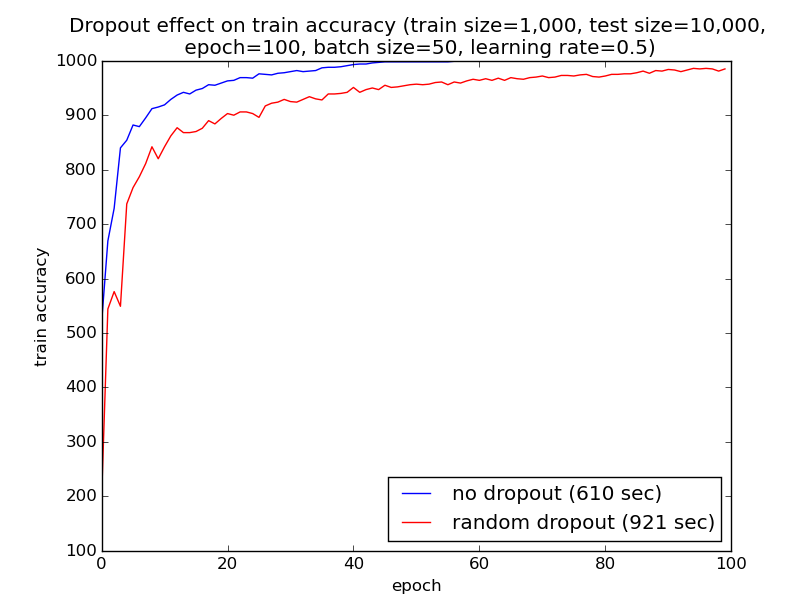
\includegraphics[width=0.7\textwidth]{../src/graphs/dropout_comparison_train_accuracy_train_1000_epoch_100_batch_50_eta_05.png}
\caption{Dropout effect on train accuracy}
\end{figure}

\begin{figure}[htp]
\centering
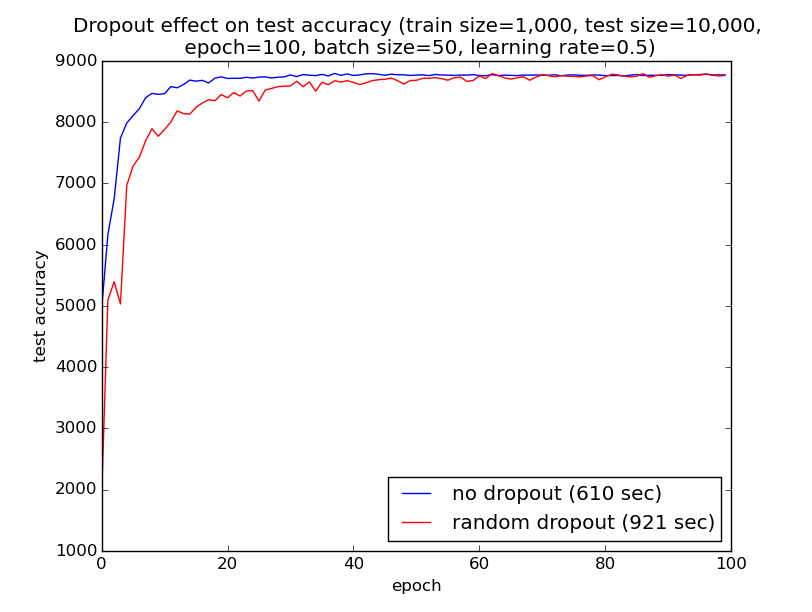
\includegraphics[width=0.7\textwidth]{../src/graphs/dropout_comparison_test_accuracy_train_1000_epoch_100_batch_50_eta_05.png}
\caption{Dropout effect on test accuracy}
\end{figure}

\begin{figure}[htp]
\centering
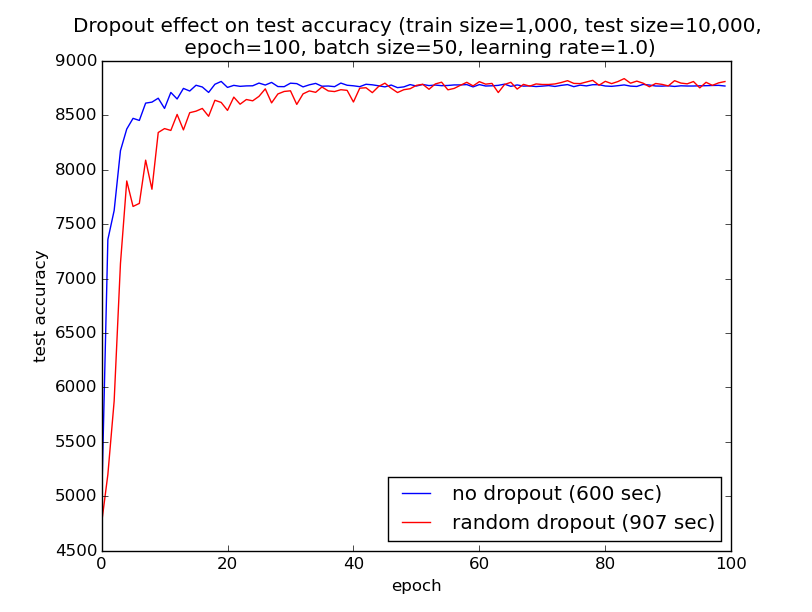
\includegraphics[width=0.7\textwidth]{../src/graphs/dropout_comparison_test_accuracy_train_1000_epoch_100_batch_50_eta_1.png}
\caption{Dropout effect on test accuracy}
\end{figure}
\newpage

\subsection{3.7. How to choose a neural network's hyper-parameters?}
\label{how-to-choose-a-neural-networks-hyper-parameters}

\subsubsection{3.7.1. Broad strategy}\label{broad-strategy}

Suppose, for example, that you're attacking MNIST for the first time.
You start out enthusiastic, but are a little discouraged when your first
network fails completely, as in the example above. The way to go is to
strip the problem down. Get rid of all the training and validation
images except images which are 0s or 1s. Then try to train a network to
distinguish 0s from 1s. Not only is that an inherently easier problem
than distinguishing all ten digits, it also reduces the amount of
training data by 80 percent, speeding up training by a factor of 5. That
enables much more rapid experimentation, and so gives you more rapid
insight into how to build a good network.

You can further speed up experimentation by stripping your network down
to the simplest network likely to do meaningful learning. If you believe
a {[}784, 10{]} network can likely do better-than-chance classification
of MNIST digits, then begin your experimentation with such a network.
It'll be much faster than training a {[}784, 30, 10{]} network, and you
can build back up to the latter.

You can get another speed up in experimentation by increasing the
frequency of monitoring. Of course, a minute isn't really very long to
wait for all training, but if you want to trial dozens of
hyper-parameter choices it's annoying. We can get feedback more quickly
by monitoring the validation accuracy more often, say, after every 1,000
training images. Furthermore, instead of using the full 10,000 image
validation set to monitor performance, we can get a much faster estimate
using just 100 validation images.

And so we can continue, individually adjusting each hyper-parameter,
gradually improving performance. Once we've explored to find an improved
value for $ \eta $, then we move on to find a good value for $
\lambda $. Then experiment with a more complex architecture, say a network
with 10 hidden neurons. Then adjust the values for
$ \eta $ and $ \lambda $ again. Then increase to 20 hidden neurons. And
then adjust other hyper-parameters some more.

\subsubsection{3.7.2. Learning rate}\label{learning-rate}

Suppose we run three MNIST networks with three different learning rates,
$ \eta = 0.025 $, $ \eta = 0.25 $ and $ \eta = 2.5 $, respectively.
Here's a graph showing the behaviour of the training cost as we train.

\begin{figure}[htp]
\centering
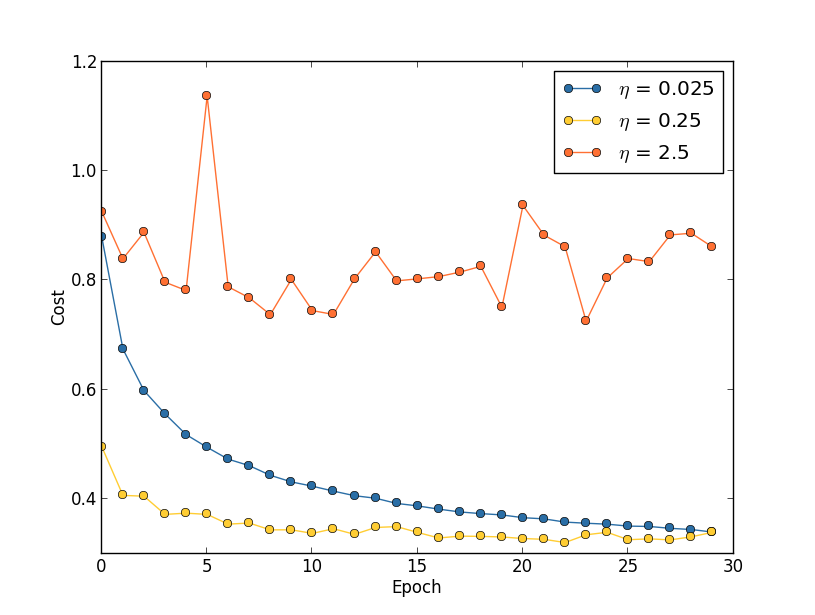
\includegraphics[width=0.7\textwidth]{./figs/multiple_eta.png}
\caption{Comparison of learning rates}
\end{figure}

With $ \eta = 0.025 $ the cost decreases smoothly until the final
epoch. With $ \eta = 0.25 $ the cost initially decreases, but after
about 20 epochs it is near saturation, and thereafter most of the
changes are merely small and apparently random oscillations. Finally,
with $ \eta = 2.5 $ the cost makes large oscillations right from the
start.

Of course, choosing $ \eta $ so small creates another problem, namely,
that it slows down stochastic gradient descent. An even better approach
would be to start with $ \eta = 0.25
$, train for 20 epochs, and then switch to $ \eta = 0.025 $. We'll
discuss such variable learning rate schedules later.

With this picture in mind, we can set $ \eta $ as follows. First, we
estimate the threshold value for $ \eta $ at which the cost on the
training data immediately begins decreasing, instead of oscillating or
increasing. This estimate doesn't need to be too accurate. You can
estimate the order of magnitude by starting with $ \eta = 0.01
$. If the cost decreases during the first few epochs, then you should successively try $
\eta = 0.1, 1.0, \ldots{} $ until you find a value for $ \eta $ where
the cost oscillates or increases during the first few epochs.
Alternately, if the cost oscillates or increases during the first few
epochs when $ \eta = 0.01 $, then try $ \eta = 0.001, 0.0001, \ldots{}
$ until you find a value for $ \eta $ where the cost decreases during
the first few epochs.

\subsubsection{3.7.3. Use early stopping to determine the number of training epochs}
\label{use-early-stopping-to-determine-the-number-of-training-epochs}

As we discussed earlier in the chapter, early stopping means that at the
end of each epoch we should compute the classification accuracy on the
validation data. When that stops improving, terminate. This makes
setting the number of epochs very simple. Furthermore, early stopping
also automatically prevents us from overfitting.

\subsubsection{3.7.4. Learning rate schedule}
\label{learning-rate-schedule}

We've been holding the learning rate $ \eta $ constant. However, it's
often advantageous to vary the learning rate. Early on during the
learning process it's likely that the weights are badly wrong. And so
it's best to use a large learning rate that causes the weights to change
quickly.

How should we set our learning rate schedule? Many approaches are
possible. The idea is to hold the learning rate constant until the
validation accuracy starts to get worse. Then decrease the learning rate
by some amount, say a factor of two or ten. We repeat this many times,
until, say, the learning rate is a factor of 1,024 (or 1,000) times
lower than the initial value. Then we terminate.

\subsubsection{3.7.5. The regularization parameter}
\label{the-regularization-parameter}

The suggestion is starting initially with no regularization $ \lambda =
0.0 $, and determining a value for $
\eta $, as above. Using that choice of $
\eta $, we can then use the validation data to select a good value for $
\lambda $. Start by trialling let' s say $ \lambda = 1.0 $ and then
increase or decrease by factors of 10, as needed to improve performance
on the validation data.

\subsubsection{3.7.6. Mini-batch size}\label{mini-batch-size}

Let' s first suppose that we're doing online learning, i.e., that we're
using a mini-batch size of 1.

The obvious worry about online learning is that using mini-batches which
contain just a single training example will cause significant errors in
our estimate of the gradient. In fact, though, the errors turn out to
not be such a problem. The reason is that the individual gradient
estimates don't need to be super-accurate. All we need is an estimate
accurate enough that our cost function tends to keep decreasing.

Summing up: Keep in mind that the heuristics described here are rules of
thumb, not rules cast in stone. You should be on the lookout for signs
that things aren't working, and be willing to experiment.

One thing that becomes clear as you read these articles and, especially,
as you engage in your own experiments, is that hyper-parameter
optimization is not a problem that is ever completely solved. There's
always another trick you can try to improve performance.

\subsection{3.8. Other techniques}
\label{other-techniques}

\subsubsection{3.8.1. Hessian technique}
\label{hessian-technique}

To begin our discussion it helps to put neural networks aside for a bit.
Instead, we're just going to consider the abstract problem of minimizing
a cost function $ C $ which is a function of many variables, $ w =
w_1, w_2, \ldots{}, $ so $ C = C(w) $. By Taylor's theorem, the cost
function can be approximated near a point $ w $ by

\begin{equation}
    \begin{split}
        C(w + \Delta w) =  C&(w)  + \sum_j \frac{\partial C}{\partial w_j}
        \Delta w_j \\ & + \frac{1}{2}\sum_{jk} \Delta w_j
        \frac{\partial^2 C}{\partial w_j \partial w_k} \Delta w_k + ...
    \end{split}
\end{equation}

We can rewrite this more compactly as

\begin{equation}
    C(w + \Delta w) = C(w) + \nabla C \cdot \Delta w +
    \frac{1}{2} {\Delta w}^T H \Delta w + …
\end{equation}

where $ \nabla C $ is the usual gradient vector, and $ H $ is a
matrix known as the Hessian matrix, whose $ jk^{th} $ entry is $
\partial^2 C / \partial w_j \partial w_k $. Suppose we
approximate $ C $ by discarding the higher-order terms
represented by $ \ldots{} $ above,

\begin{equation}
    C(w + \Delta w) \approx C(w) + \nabla C \cdot \Delta w +
    \frac{1}{2} {\Delta w}^T H \Delta w
\end{equation}

Using calculus we can show that the expression on the right-hand side
can be minimized by choosing

\begin{equation}
    \Delta w = −H^{−1} \nabla C
\end{equation}

In practice, (53) is only an approximation, and it's better to take
smaller steps. We do this by repeatedly changing $ w $ by an amount $
\Delta w = -\eta H^{−1} \nabla C $, where $ \eta $ is known as
the learning rate.

This approach to minimizing a cost function is known as the Hessian
technique or Hessian optimization. There are theoretical and empirical
results showing that Hessian methods converge on a minimum in fewer
steps than standard gradient descent. In particular, by incorporating
information about second-order changes in the cost function it's
possible for the Hessian approach to avoid many pathologies that can
occur in gradient descent. Furthermore, there are versions of the
backpropagation algorithm which can be used to compute the Hessian.

Unfortunately, while it has many desirable properties, it has one very
undesirable property: the Hessian matrix is very big. Suppose you have a
neural network with $ 10^7 $ weights and biases. Then the
corresponding Hessian matrix will contain $ 10^7 \times 10^7 =
10^{14} $ entries. That's a lot of entries to compute, especially
when you're going to need to invert the matrix as well! That makes
Hessian optimization difficult to apply in practice.

\subsubsection{3.8.2. Momentum-based gradient descent}
\label{momentum-based-gradient-descent}

Unlike Hessian technique momentum-based gradient descent avoids large
matrices of second derivatives. The momentum technique modifies gradient
descent in two ways that make it more similar to the physical picture.
First, it introduces a notion of ``velocity'' for the parameters we're
trying to optimize. The gradient acts to change the velocity, not
(directly) the ``position'', in much the same way as physical forces
change the velocity, and only indirectly affect position. Second, the
momentum method introduces a kind of friction term, which tends to
gradually reduce the velocity.

We introduce velocity variables $ v = v_1, v_2, \ldots{} $ one for
each corresponding $ w_j $ variable. Then we replace the gradient
descent update rule $ w \to w′ = w - \eta \nabla C $ by

\begin{equation}
    \begin{split}
        v & \to \mu v - \eta \nabla C \\
        w & \to  w + v
    \end{split}
\end{equation}

In these equations, $ \mu $ is a hyper-parameter which controls the
amount of damping or friction in the system. To understand the meaning
of the equations it's helpful to first consider the case where $ \mu =
1 $, which corresponds to no friction. When that's the case,
inspection of the equations shows that the ``force''
$ \nabla C $ is now modifying the velocity, $ v $, and
the velocity is controlling the rate of change of $ w $.
Intuitively, we build up the velocity by repeatedly adding
gradient terms to it. That means that if the gradient is in
(roughly) the same direction through several rounds of learning,
we can build up quite a bit of steam moving in that direction.
Think, for example, of what happens if we're moving straight down a slope.
With each step the velocity gets larger down the slope, so we move more and
more quickly to the bottom of the valley. This can enable the momentum
technique to work much faster than standard gradient descent.
Of course, a problem is that once we reach the bottom of the valley we will overshoot.
Or, if the gradient should change rapidly, then we could find ourselves moving
in the wrong direction. That's the reason for the $ \mu $
hyper-parameter in (54). To be a little more precise, you should
think of $ 1 − \mu $ as the amount of friction in the system. When $
\mu = 1 $, as we've seen, there is no friction, and the velocity
is completely driven by the gradient $ \nabla C $.
By contrast, when $ \mu = 0 $ there's a lot of friction,
the velocity can't build up, and Equation (54) reduce to the
usual equation for gradient descent, $ w\to w′ = w − \eta \nabla C $

It' s avoided naming the hyper-parameter $ \mu $ up to now. The reason
is that the standard name for $ \mu $ is badly chosen: it's called the
momentum co-efficient. This is potentially confusing, since $ \mu $ is
not at all the same as the notion of momentum from physics. Rather, it
is much more closely related to friction.

A nice thing about the momentum technique is that it takes almost no
work to modify an implementation of gradient descent to incorporate
momentum. We can still use backpropagation to compute the gradients,
just as before, and use ideas such as sampling stochastically chosen
mini-batches. In this way, we can get some of the advantages of the
Hessian technique, using information about how the gradient is changing.
In practice, the momentum technique is commonly used, and often speeds
up learning.

\subsection{3.9. Other models of artificial neuron}
\label{other-models-of-artificial-neuron}

Up to now we've built our neural networks using sigmoid neurons. In
practice, networks built using other model neurons sometimes outperform
sigmoid networks.

Perhaps the simplest variation is the $ \tanh $ (pronounced ``tanch'')
neuron, which replaces the sigmoid function by the hyperbolic tangent
function. The output of a $ \tanh $ neuron with input $ x
$, weight vector $ w $, and bias $ b $ is given by

\begin{equation}
    \tanh(w \cdot x + b)
\end{equation}

Recall that the $ \tanh $ function is defined by

\begin{equation}
    \tanh(z) \equiv \frac{e^z − e^{-z}}{e^z + e^{-z}}
\end{equation}

With a little algebra it can easily be verified that

\begin{equation}
    \sigma(z) = \frac{1 + \tanh(z / 2)}{2}
\end{equation}

that is, $ \tanh $ is just a rescaled version of the sigmoid function.
We can also see graphically that the $ \tanh $ function has the same
shape as the sigmoid function,

\begin{figure}[htp]
\centering
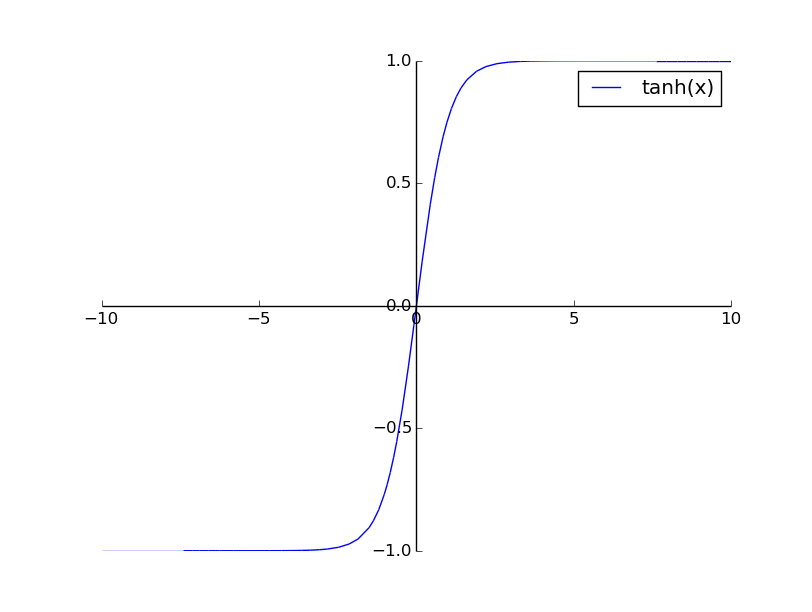
\includegraphics[width=0.7\textwidth]{./figs/tanh_function.png}
\caption{Tanh function}
\end{figure}

One difference between tanh neurons and sigmoid neurons is that the
output from tanh neurons ranges from $ -1 $ to $ 1 $, not $ 0 $ to
$ 1 $. This means that if you're going to build a network based on
tanh neurons you may need to normalize your outputs\cite{ref3}.

If some of the input activations have different signs, replace the
sigmoid by an activation function, such as $ \tanh $,
which allows both positive and negative activations. Indeed, because $ \tanh $
is symmetric about zero, $ \tanh(−z) = −tanh(z) $.

Another variation on the sigmoid neuron is the rectified linear neuron
or rectified linear unit. The output of a rectified linear unit with
input $ x $, weight vector $ w $, and bias $ b $ is given by

\begin{equation}
    \max(0, w \cdot x + b)
\end{equation}

Graphically, the rectifying function $ \max(0, z) $ looks like this:

\begin{figure}[htp]
\centering
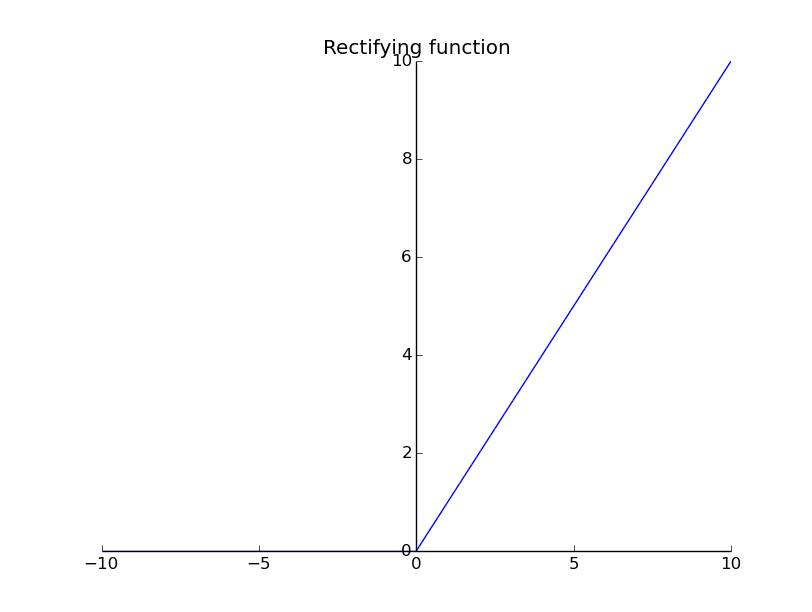
\includegraphics[width=0.7\textwidth]{./figs/rectifying_function.png}
\caption{Rectifying function}
\end{figure}

Like the sigmoid and tanh neurons, rectified linear units can be used to
compute any function, and they can be trained using ideas such as
backpropagation and stochastic gradient descent.
\newpage
\begin{thebibliography}{99}
\bibitem{ref1}
Nielsen, Michael (2015). Neural Networks and Deep Learning
\bibitem{ref2}
Nielsen, Michael (2012-2015). URL: https://github.com/mnielsen/neural-networks-and-deep-learning
\bibitem{ref3}
Olah, Christopher (2014). URL: https://colah.github.io/posts/2014-03-NN-Manifolds-Topology/
\end{thebibliography}

\end{document}
